\chapter{Deep learning applied to glacier evolution modelling}
\label{chap:methods}

\begin{flushright}
\begin{small}
\textit{All models are wrong, but some are useful.}\\
George Box
\end{small}
\end{flushright}

\section*{Preface}

\section{Abstract}
We present a novel approach to simulate and reconstruct annual glacier-wide surface mass balance (SMB) series based on a deep artificial neural network (\textit{i.e.} deep learning). This method has been included as the SMB component of an open-source regional glacier evolution model. While most glacier models tend to incorporate more and more physical processes, here we take an alternative approach by creating a parameterized model based on data science. Annual glacier-wide SMBs can be simulated from topo-climatic predictors using either deep learning or Lasso (regularized multilinear regression), whereas the glacier geometry is updated using a glacier-specific parameterization. We compare and cross-validate our nonlinear deep learning SMB model against other standard linear statistical methods on a dataset of 32 French alpine glaciers. Deep learning is found to outperform linear methods, with improved explained variance (up to +64\% in space and +108\% in time) and accuracy (up to +47\% in space and +58\% in time), resulting in an estimated \(r^2\) of 0.77 and RMSE of 0.51 m.w.e. Substantial nonlinear structures are captured by deep learning, with around 35\% of nonlinear behaviour in the temporal dimension. For the glacier geometry evolution, the main uncertainties come from the ice thickness data used to initialize the model. These results should encourage the use of deep learning in glacier modelling as a powerful nonlinear tool, capable of capturing the nonlinearities of the climate and glacier systems, that can serve to reconstruct or simulate SMB time series for individual glaciers in a whole region for past and future climates. 


\section{Introduction} \label{methods:intro}

Glaciers are arguably one of the most important icons of climate change, being climate proxies which can depict the evolution of climate for the global audience \citep{ipcc_climate_2018}. In the coming decades, mountain glaciers will be some of the most important contributors to sea level rise and will most likely drive important changes in the hydrological regime of glaciarized catchments \citep{beniston_european_2018, vuille_rapid_2018, hock_glaciermip_2019}. The reduction in ice volume may produce an array of hydrological, ecological and economic consequences in mountain regions which requires to be properly predicted. These consequences will strongly depend on the future climatic scenarios, which will determine the timing and magnitude for the transition of hydrological regimes \citep{huss_global-scale_2018}. Understanding these future transitions is key for societies to adapt to future hydrological and climate configurations. 

Glacier and hydro-glaciological models can help answer these questions, giving several possible outcomes depending on multiple climate scenarios. (a) Surface mass balance (SMB) and (b) glacier dynamics both need to be modelled to understand glacier evolution on regional and sub-regional scales. Models of varying complexity exist for both processes. In order to model these processes at large scale (\textit{i.e.} on several glaciers at a catchment scale), some compromises need to be made, which can be approached in different ways:

(a) Regarding SMB:

\begin{enumerate}
\item Empirical models, like the temperature-index model \citep[e.g.][]{hock_temperature_2003}, simulate glacier SMB through empirical relationships between air temperature and melt and snow accumulation. 
\item Statistical or machine learning models describe and predict glacier SMB based on statistical relationships found in data from a selection of topographical and climate predictors \citep[e.g.][]{martin_correlation_1974, steiner_application_2005}.
\item Physical and Surface Energy Balance (SEB) models take into account all energy exchanges between the glacier and the atmosphere, and can simulate the spatial and temporal variability of snowmelt and the changes in albedo \citep[e.g.][]{gerbaux_surface_2005}.
\end{enumerate}

(b) Regarding glacier dynamics:

\begin{enumerate}
\item Parameterized models do not explicitly resolve any physical processes, but implicitly take them into account using parameterizations, based on statistical or empirical relationships, in order to modify the glacier geometry. This type of models range from very simple statistical models \citep[e.g.][]{carlson_accounting_2014} to more complex ones based on different approaches, such as a calibrated equilibrium-line altitude (ELA) model \citep[e.g.][]{zemp_alpine_2006}, a glacier retreat parameterization specific for glacier size groups \citep{huss_new_2015} or volume/length-area scaling \citep[e.g.][]{marzeion_past_2012, radic_regional_2014}. 
\item Process-based models, like GloGEMflow \citep[e.g.][]{zekollari_modelling_2019} and OGGM \citep[e.g.][]{maussion_open_2019}, approximate a number of glacier physical processes involved in ice flow dynamics using the shallow ice approximation. 
\item Physics-based models, like the finite elements Elmer/Ice model \citep[e.g.][]{gagliardini_capabilities_2013}, approach glacier dynamics by explicitly simulating physical processes and solving the full Stokes equations \citep[e.g.][]{jouvet_numerical_2009, reveillet_simulations_2015}. 
\end{enumerate}

At the same time, the use of these different approaches strongly depend on available data, whose spatial and temporal resolutions have an important impact on the results’ quality and uncertainties \citep[e.g.,][]{reveillet_relative_2018}. Parameterized glacier dynamics models and empirical and statistical SMB models require a reference or training dataset to calibrate the relationships, which can then be used for projections with the hypothesis that relationships remain stationary in time. On the contrary, process-based and specially physics-based glacier dynamics and SMB models have the advantage of representing physical processes, but they require larger datasets at higher spatial and temporal resolutions with a consequently higher computational cost \citep{reveillet_relative_2018}. For SMB modelling, meteorological reanalyses provide an attractive alternative to sparse point observations, although their spatial resolution and suitability to complex high-mountain topography are often not good enough for high-resolution physics-based glacio-hydrological applications. However, parameterized models are much more flexible, equally dealing with fewer and coarser meteorological data as well as the state of the art reanalyses, which allows to work at resolutions much closer to glaciers’ scale and to reduce uncertainties. The current resolution of climate projections is still too low to adequately drive most glacier physical processes, but the ever-growing datasets of historical data are paving the way for the training of parameterized machine learning models. 

In glaciology, statistical models have been applied for more than half a century, starting with simple multiple linear regressions on few meteorological variables \citep{hoinkes_glacier_1968, martin_correlation_1974}. Statistical modelling has made enormous progress in the last decades, specially thanks to the advent of machine learning. Compared to other fields in geosciences, such as oceanography \citep[e.g.,][]{ducournau_deep_2016, lguensat_eddynet:_2018}, climatology \citep[e.g.,][]{rasp_deep_2018, jiang_deep_2018} and hydrology \citep[e.g.,][]{marcais_prospective_2017, shen_transdisciplinary_2018}, we believe that the glaciological community has not yet exploited the full capabilities of these approaches. Despite this fact, a number of studies have taken steps towards statistical approaches. \citet{steiner_application_2005} pioneered the very first study to use artificial neural networks (ANNs) in glaciology to simulate mass balances of the Grosse Aletschgletscher in Switzerland. They showed that a nonlinear model is capable of better simulating glacier mass balances compared to a conventional stepwise multiple linear regression. Furthermore, they found a significant nonlinear part within the climate/glacier mass balance relationship. This work was continued in \citet{steiner_sensitivity_2008} and \citet{nussbaumer_reseau_2012} for the simulation of glacier length instead of mass balances. Later on, \citet{maussion_enso_2015} developed an empirical statistical downscaling tool based on machine learning in order to retrieve glacier surface energy and mass balance (SEB/SMB) fluxes from large-scale atmospheric data. They used different machine learning algorithms, but all of them were linear, which are not necessarily the most suitable for modelling the nonlinear climate system \citep{houghton_climate_2001}. Nonetheless, more recent developments in the field of machine learning and optimization enabled the use of deeper network structures than the 3-layer ANN of \citet{steiner_application_2005}. These deeper ANNs, which remain unexploited in glaciology, are capable of capturing more nonlinear structures in the data even for relatively small datasets  \citep{ingrassia_neural_2005, olson_modern_2018}. 

Here, we present a parameterized regional open-source glacier model: the ALpine Parameterized Glacier Model \cite[ALPGM,][]{bolibar_jordibolibar/alpgm:_2019}. When most glacier evolution models tend to incorporate more and more physical processes in SMB or ice dynamics \citep[e.g.,][]{maussion_open_2019, zekollari_modelling_2019}, ALPGM takes an alternative approach based on data science for SMB modelling and parameterizations for glacier dynamics simulation. ALPGM simulates annual glacier-wide SMB and the evolution of glacier volume and surface area over time scales from a few years to a century at a regional scale. Glacier-wide SMBs are computed using a deep ANN, fed by several topographical and climatic variables, an approach which is compared to different linear methods in the present paper. In order to distribute these annual glacier-wide SMBs and to update the glacier geometry, a refined version of the $\Delta$h methodology \citep[e.g.,][]{huss_modelling_2008} is used, for which we dynamically compute glacier-specific $\Delta$h functions. In order to validate this approach, we use a case study with 32 French alpine glaciers for which glacier-wide annual SMBs are available over the period 1984-2014 and 1959-2015 for certain glaciers. High resolution meteorological reanalyses for the same time period are used \citep[SAFRAN,][]{durand_reanalysis_2009} while the initial ice thickness distribution of glaciers are taken from \citet{farinotti_consensus_2019}, for which we performed a sensitivity analysis based on field observations.

In the next section, we present an overview of the proposed glacier evolution model framework with a detailed description of the two components used to simulate the annual glacier-wide SMB and the glacier geometry update. Then, a case study using French alpine glaciers is presented, which enables to illustrate an example of application of the proposed framework including a rich dataset, the parameterized functions, as well as the results and their performance. In the end, several aspects regarding machine and deep learning modelling in glaciology are discussed, from which we make some recommendations and draw the final conclusions.


\section{Model overview and methods} \label{methods:methods}

In this section we present an overview of the ALPGM glacier model. Moreover, the two components of this model are presented in detail: the Glacier-wide SMB Simulation component and the Glacier Geometry Update component.

\subsection{Model overview and workflow} \label{methods:methods:workflow}

ALPGM is an open-source glacier model coded in Python. The source code of the model is accessible in the project repository (see Code availability). It is structured in multiple files which execute specific separate tasks. The model can be divided into two main components: (1) the Glacier-wide SMB Simulation and (2) the Glacier Geometry Update. The Glacier-wide SMB Simulation component is based on machine learning, taking both meteorological and topographical variables as inputs. The Glacier Geometry Update component generates the glacier-specific parameterized functions and modifies annually the geometry of the glacier (\textit{e.g.} ice thickness distribution, glacier outline) based on the glacier-wide SMB models generated by the Glacier-wide SMB simulation component.

\begin{figure*}[t]
\centering
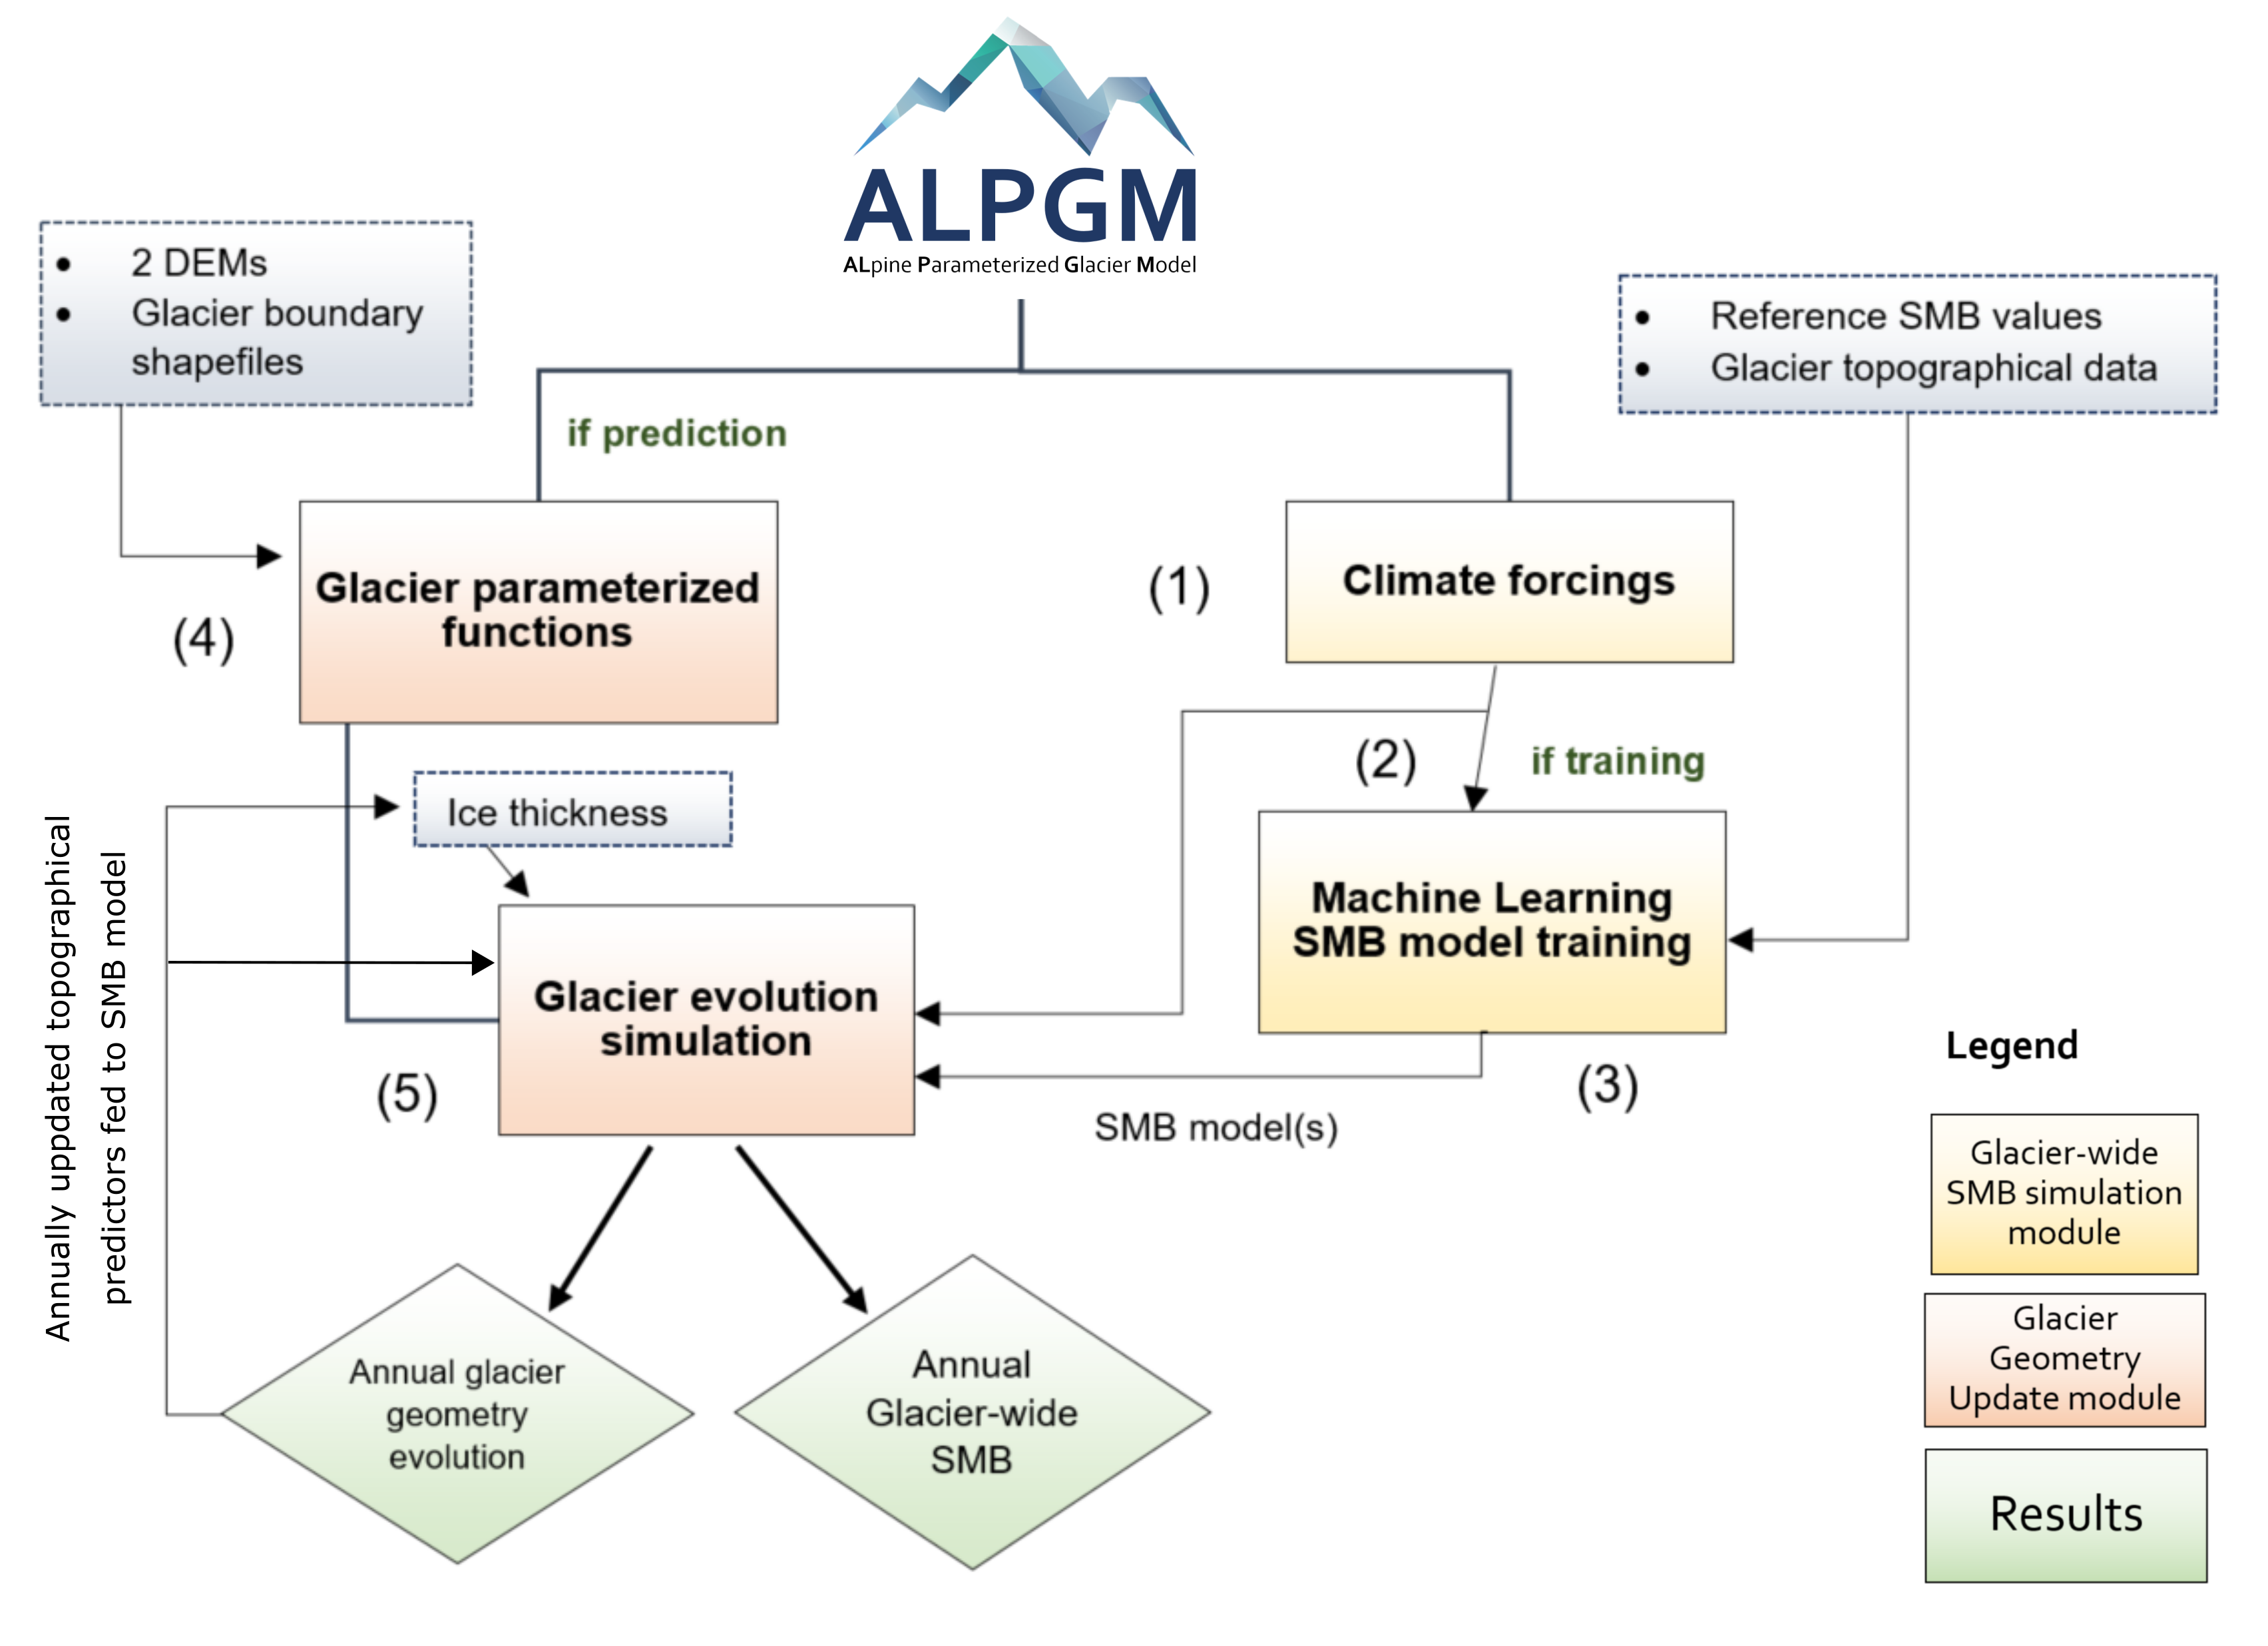
\includegraphics[width=14cm]{Figures/methods/Figure_1.png}
\caption{ALPGM structure and workflow}
\label{methods:fig1}
\end{figure*}

Figure \ref{methods:fig1} presents ALPGM’s basic workflow. The workflow execution can be configured via the model interface, allowing to run or skip any of the following steps:

\begin{enumerate}
\item The meteorological forcings are preprocessed in order to extract the necessary data closest to each glacier’s centroid. The meteorological features are stored in intermediate files in order to reduce computation times for future runs, automatically skipping this preprocessing step when the files have already been generated.
\item The SMB machine learning component retrieves the preprocessed climate predictors from the stored files, retrieves the topographical predictors from the multitemporal glacier inventories, and then it assembles the training dataset by combining all the necessary topo-climatic predictors. A machine learning algorithm is chosen for the SMB model, which can be loaded from a previous run or it can be trained again with a new dataset. Then, the SMB model(s) are trained with the full topo-climatic dataset. These model(s) are stored in intermediate files, allowing to skip this step for future runs.
\item Performances of the SMB models can be evaluated with a leave-one-glacier-out (LOGO) or a leave-one-year-out (LOYO) cross-validation. This step can be skipped when using already established models. Basic statistical performance metrics are given for each glacier and model, as well as plots with the simulated cumulative glacier-wide SMBs compared to their reference values with uncertainties for each of the glaciers from the training dataset.
\item The Glacier Geometry Update component starts with the generation of the glacier specific parameterized functions, using a raster containing the difference of the two pre-selected digital elevation models (DEMs) covering the study area for two separate dates, as well as the glacier contours. These parameterized functions are then stored in individual files to be used in the final simulations.
\item Once all previous steps have been run, the glacier evolution simulations are launched. For each glacier, the initial ice thickness and DEM rasters and the glacier geometry update function are retrieved. Then, in a loop, for every glacier and year, the topographical data is computed from these raster files. The climate predictors at the glacier’s current centroid are retrieved from the climate data (e.g. reanalysis or projections) and with all this data the input topo-climatic data for the glacier-wide SMB model is assembled. Afterwards, the glacier-wide SMB for this glacier and year is simulated, which combined with the glacier-specific geometry update function allows to update the glacier’s ice thickness and DEM rasters. This process is repeated in a loop, therefore updating the glacier’s geometry with an annual timestep and taking into account the glacier’s morphological and topographical changes in the glacier-wide SMB simulations. For the simulation of the following year’s SMB, the previously updated ice thickness and DEM rasters is used to re-compute the topographical parameters, which in turn are used as input topographical predictors for the glacier-wide SMB machine learning model.  If all the ice thickness raster pixels of a glacier become zero, the glacier is considered as disappeared and is removed from the simulation pipeline. For each year, multiple results are stored in data files as well as the raster DEM and ice thickness values for each glacier. 
\end{enumerate}

\subsection{Glacier-wide surface mass balance simulation} \label{methods:methods:SMB}
Annual glacier-wide SMBs are simulated using machine learning. Due to the regional characteristics and specificities of topographical and climate data, this glacier-wide SMB modelling method is, for now, a regional approach.

\subsubsection{Selection of explanatory topographical and climatic variables} 

In order to narrow down which topographical and climatic variables best explain glacier-wide SMB in a given study area, a literature review as well as a statistical sensitivity analysis are performed. Typically used topographical predictors are longitude, latitude, glacier slope and mean altitude. As for meteorological predictors, cumulative positive degree days (CPDD), but also mean monthly temperature, snowfall and possibly other variables that influence the surface energy budget are often used in the literature. Examples of both topographic and meteorological predictors can be found in the case study in Sect. \ref{methods:case_study}. A way to prevent biases when making predictions with different climate data is to work with anomalies, calculated as differences of the variable with respect to its average value over a chosen reference period. 

For the machine learning training, the relevant predictors must be selected, so we perform a sensitivity study of the annual glacier-wide SMB to topographical and climatic variables over the study training period. This can be performed with individual linear regressions between each variable and glacier-wide SMB data. After identification of the topographical and climatic variables that can potentially explain annual glacier-wide SMB variability for the region of interest, a training dataset is built. An effective way of expanding the training dataset in order to dig deeper into the available data is to combine the climatic and topographical input variables \citep{weisberg_applied_2014}. Such combinations can be expressed following equation \ref{eq:1}

\begin{equation} \label{eq:1}
SMB_{g, y}=f(\hat{\Omega}, \hat{C})+\varepsilon_{g, y}
\end{equation}

Where $\hat{\Omega}$ is a vector of the selected topographical predictors, $\hat{C}$ is a vector with the selected climatic features and $\varepsilon_{g, y}$ is the residual error for each annual glacier-wide SMB value, $SMB_{g, y}$.

Once the training dataset is created, different algorithms $f$ (two linear and one nonlinear, for the case of this study) can be chosen to create the SMB model: (1) OLS (Ordinary Least Squares) all-possible multiple linear regressions; (2) Lasso (Least absolute shrinkage and selection operator) \citep{tibshirani_regression_1996}; and (3) a deep Artificial Neural Network (ANN). ALPGM uses some of the most popular machine learning Python libraries: StatsModels \citep{seabold_statsmodels:_2010}, Scikit-learn \citep{pedregosa_scikit-learn:_2012} and Keras \citep{chollet_keras_2015} with a TensorFlow backend. The overall workflow of the machine learning glacier-wide SMB model production in ALPGM is summarized in Fig. \ref{methods:fig2}.  

\begin{figure}[t]
\centering
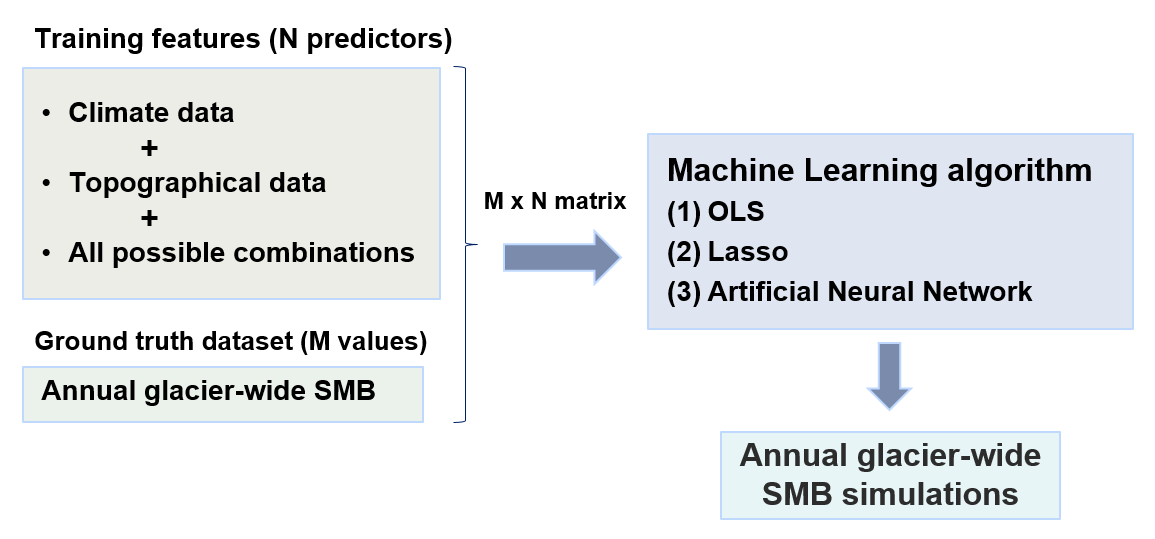
\includegraphics[width=9cm]{Figures/methods/Figure_2.png}
\caption{Glacier-wide SMB simulation component workflow. Machine learning models are dynamically created based on training data}
\label{methods:fig2}
\end{figure}

\subsubsection{All-possible multiple linear regressions} \label{methods:methods:ols}

With the ordinary least squares (OLS) all-possible multiple linear regressions, we attempt to find the best subset of predictors in Eq. \ref{eq:1} based on the resulting \(r^2\) adjusted, while at the same time avoiding overfitting \citep{hawkins_problem_2004} and collinearity, and limiting the complexity of the model. As its name indicates, the goal is to minimize the residual sum of squares for each subset of predictors \citep{hastie_elements_2009}. $n$ models are produced by selecting all possible subsets of $k$ predictors. It is advisable to narrow down the number of predictors for each subset in the search to reduce the computational cost. Models with low performance are filtered out, keeping only models with highest \(r^2\) adjusted possible, a variance inflation factor ($VIF$) < 1.2 and a p-value < 0.01/$n$ (in order to ensure the Bonferroni correction). Retained models are combined by averaging their predictions, thereby avoiding the pitfalls related to stepwise single model selection \citep{whittingham_why_2006}. These criteria ensure that the models explain as much variability as possible, avoid collinearity and are statistically significant. 

\subsubsection{Lasso} \label{methods:methods:lasso}

The Lasso (Least absolute shrinkage and selection operator) \citep{tibshirani_regression_1996} is a shrinkage method which attempts to overcome the shortcomings of the simpler step-wise and all-possible regressions. In these two classical approaches, predictors are discarded in a discrete way, giving subsets of variables which have the lowest prediction error. However, due to its discrete selection, these different subsets can exhibit high variance, which does not reduce the prediction error of the full model. The Lasso performs a more continuous regularization by shrinking some coefficients and setting others to zero, thus producing more interpretable models \citep{hastie_elements_2009}. Because of its properties, it strikes a balance between subset selection (like all-possible regressions) and Ridge regression \citep{hoerl_ridge_1970}. All input data is normalized by removing the mean and scaling to unit variance. In order to determine the degree of regularisation applied to the coefficients used in the linear OLS regression, an alpha parameter needs to be chosen using cross-validation. ALPGM performs different types of cross-validations to choose from: the Akaike Information Criterion (AIC), the Bayes Information Criterion (BIC) and a classical cross-validation with iterative fitting along a regularization path (used in the case study). Alternatively, a Lasso model with Least Angle Regression, also known as Lasso Lars \citep{tibshirani_least_2004}, can also be chosen with a classical cross-validation. 

\subsubsection{Deep artificial neural networks} \label{methods:methods:ann}

Artificial neural networks (ANNs) are nonlinear statistical models inspired by biological neural networks \citep{fausett_fundamentals_1994, hastie_elements_2009}. A neural network is characterized by: (1) the architecture or pattern of connections between units and the number of layers (input, output and hidden layers); (2) the optimizer: which is the method for determining the weights of the connections between units; and (3) its (usually nonlinear) activation functions \citep{fausett_fundamentals_1994}. When ANNs have more than one hidden layer (\textit{e.g.} Fig. \ref{methods:fig3}), they are referred to as deep ANNs or deep learning. The description of neural networks is beyond the scope of this study, so for more details and a full explanation please refer to \citet{fausett_fundamentals_1994}, \citet{hastie_elements_2009}, as well as \citet{steiner_application_2005, steiner_sensitivity_2008} where the reader can find a thorough introduction to the use of ANNs in glaciology. ANNs gained recent interest thanks to improvements of optimization algorithms enabling the training of deep neural networks, that lead to better representation of complex data patterns. As their learnt parameters are difficult to interpret, ANN are adequate tools when the quality of predictions prevails over the interpretability of the model (the latter likely involving causal inference, sensitivity testing or modelling of ancillary variables). This is precisely the case in our study context here, where abundant knowledge about glacier physics further helps choosing adequate variables as input to deep learning. Their ability to model complex functions of the input parameters makes them particularly suitable for modelling complex nonlinear systems such as the climate system \citep{houghton_climate_2001} and glacier systems \citep{steiner_application_2005}.

ALPGM uses a feedforward fully-connected ANN (Fig. \ref{methods:fig3}). In such an architecture, the processing units - or neurons - are grouped into layers where all the units of a given layer are fully connected to all units of the next layer. The flow of information is directional, from the input layer (\textit{i.e.}. in which each neuron corresponds to one of the N explanatory variables) to the output neuron (\textit{i.e.}. corresponding to the target variable of the model, the SMB). For each connection of the ANN, weights are initialized in a random fashion following a specific distribution (generally centred around 0). In each unit of each hidden layer, the weighted values are summed before going through a nonlinear activation function, responsible for introducing the nonlinearities in the model. Using a series of iterations known as epochs, the ANN will try to minimize a specific loss function (the mean squared error (MSE) in our case) comparing the processed values of the output layer with the ground truth ($y$). In order to avoid falling into local minima of the loss function, some regularisation is needed to prevent the ANN from overfitting \citep{hastie_elements_2009}.  To prevent overfitting during the training process (\textit{i.e.}. to increase the ability of the model to generalize to new data), we used a classical regularization method called dropout, consisting in training iteratively smaller subparts of the ANN by randomly disconnecting a certain amount of connections between units. The introduction of Gaussian noise at the input of the ANN also helped to generalize, as it performs a similar effect to data augmentation. The main consequence of regularisation is generalization, for which the produced model is capable of better adapting to different configurations of the input data. 

\begin{figure*}[t]
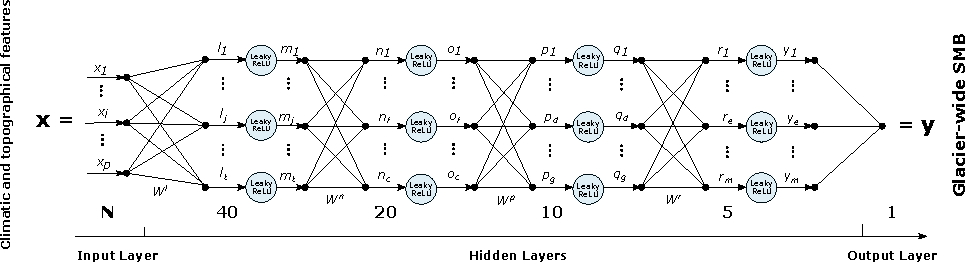
\includegraphics[width=15cm]{Figures/methods/Figure_3.pdf}
\caption{Deep Artificial Neural Network architecture used in ALPGM. The numbers indicate the number of neurons in each layer}
\label{methods:fig3}
\end{figure*}

The hyperparameters used to configure the ANN are determined using cross-validation, in order to find the best performing combination of number of units, hidden layers, activation function, learning rate and regularisation method. Due to the relatively small size of our dataset, we encountered the best performances with a quite small deep ANN, with a total of 6 layers (4 hidden layers) with a ($N$, 40, 20, 10, 5, 1) architecture (Fig. \ref{methods:fig3}), where $N$ is the number of selected features. Since the ANN already performs all the possible combinations between features (predictors), we use a reduced version of the training matrix from Eq. \ref{eq:1}, with no combination of climatic and topographical features. Due to the relatively small size of the architecture, the best dropout rates are small \citep{srivastava_dropout:_2014}, and range between 0.3 and 0.01 depending on the number of units of each hidden layer. Leaky ReLUs have been chosen as the activation function, because of their widespread reliability and the fact they help prevent the “dead ReLU” problem, where certain neurons can stop “learning” \citep{xu_empirical_2015}. The He uniform initialization \citep{he_delving_2015} has been used as it is shown to work well with Leaky ReLUs, and all unit bias were initialized to zero. In order to optimize the weights of the gradient descent, we used the RMSprop optimizer, for which we fine-tuned the learning rate, obtaining the best results at 0.0005 in space and 0.02 in time. Each batch was normalized before applying the activation function in order to accelerate the training \citep{ioffe_batch_2015}. 

Like for many other geophysical processes found in nature, extreme annual glacier-wide SMB values occur much less often than average values, approximately following an unbounded Gumbel-type distribution \citep{thibert_causes_2018}. From a statistical point of view, this means that ANN will “see” few extreme values and will accord less importance to them. For future projections in a warmer climate, extreme positive glacier-wide SMB balances should not be the main concern of glacier models. However, extreme negative annual glacier-wide SMB values should likely increase in frequency, so it is in the modeller’s interest to reproduce them as well as possible. Setting the sample weights as the inverse of the probability density function during the ANN training can partly compensate for the imbalance of a dataset. This boosts the performance of the model for the extreme values, at the cost of sacrificing some performance on more average values, which can be seen as a \(r^2\)/RMSE trade-off (Fig. \ref{methods:fig6} and \ref{methods:fig9} from the case study). The correct setting of the sample weights allows the modeller to adapt the ANN to each dataset and application. 

\subsection{Glacier geometry update} \label{methods:methods:deltah}

Since the first component of ALPGM simulates annual glacier-wide SMBs, these changes in mass need to be redistributed over the glacier surface-area in order to reproduce glacier dynamics. This redistribution is applied using the $\Delta$h parameterization. The idea was first developed by \citet{johannesson_timescale_1989} and then adapted and implemented by \citet{huss_modelling_2008}. The main idea behind it is to use two or more DEMs covering the study area. These DEMs should have dates covering a period long enough (which will be later discussed in detail). By subtracting them, the changes in glacier surface elevation over time can be computed, which corresponds to a change in thickness (considering no basal erosion). Then, these thickness changes are normalized and considered as a function of the normalized glacier altitude. This $\Delta$h function is specific for each glacier and represents the normalized glacier thickness evolution over its altitudinal range. One advantage of such a parametrized approach is that it implicitly considers the ice flow which redistributes the mass from the accumulation to the ablation area. In order to make the glacier volume evolve in a mass-conserving fashion, we apply this function to the annual glacier-wide SMB values in order to scale and distribute its change in volume. 

As discussed in \citet{vincent_future_2014}, the time period between the two DEMs used to calibrate the method needs to be long enough to show important ice thickness differences. The criteria will of course depend on each glacier and each period, but it will always be related to the achievable signal-to-noise ratio. \citet{vincent_future_2014} concluded that for their study on the Mer de Glace glacier (28.8 \(km^2\), mean altitude = 2868 m.a.s.l.) in the French Alps, the 2003-2008 period was too short, due to the delayed response of glacier geometry to a change in surface mass balance. Indeed, the results for that 5-year period diverged from the results from longer periods. Moreover, the period should be long enough to be representative of the glacier evolution, which will often encompass periods with strong ablation and others with no retreat or even with positive SMBs. 

Therefore, by subtracting the two DEMs, the ice thickness difference is computed for each specific glacier. These values can then be classified by altitude, thus obtaining an average glacier thickness difference for each pixel altitude. As a change to previous studies \citep{vincent_future_2014, huss_new_2015, hanzer_projected_2018, vincent_declin_2019}, we no longer work with altitudinal transects, but with individual pixels. In order to filter noise and artefacts coming from the DEM raster files, different filters are applied to remove outliers and pixels with unrealistic values, namely at the border of glaciers or where the surface slopes are high (refer to Supplements for detailed information). Our methodology thus allows to better exploit the available spatial information based on its quality, and not on arbitrary location within transects. 

\section{Case study: French alpine glaciers} \label{methods:case_study}
\subsection{Data} \label{methods:case_study:data}

All data used in this case study is based on the French Alps (Fig. \ref{methods:fig4}), located in the westernmost part of the European Alps, between 5.08° and 7.67°E, and 44° and 46°13’N. This region is particularly suited for the validation of a glacier evolution model because of the wealth of available data. Moreover, ALPGM has been developed as part of a hydro-glaciological study to understand the impact of the retreat of French alpine glaciers in the Rhône river catchment (97,800 \(km^2\)). 

\subsubsection{Glacier-wide surface mass balance }

An annual glacier-wide SMB dataset, reconstructed using remote sensing based on changes in glacier volume and the snow line altitude, is used \citep{rabatel_spatio-temporal_2016}. This dataset is constituted by annual glacier-wide SMB values for 30 glaciers in the French Alps (Fig. \ref{methods:fig4}) for 31 years, between 1984-2014. The great variety in topographical characteristics of the glaciers included in the dataset, with a good coverage of the three main clusters or groups of glaciers in the French Alps (Fig. \ref{methods:fig4}), makes them an ideal training dataset for the model. Each of the clusters represents a different setup of glaciers with different contrasting latitudes (Écrins and Mont-Blanc), longitudes (Écrins and Vanoise), glacier size (smaller glaciers in Écrins and Vanoise $vs$ larger ones in Mont-Blanc) and climatic characteristics with a Mediterranean influence towards the south of the study region. For more details regarding this dataset refer to \citet{rabatel_spatio-temporal_2016}. Data from the Mer de Glace, Saint-Sorlin, Sarennes and Argentière glaciers is also used, coming from field observations from the GLACIOCLIM observatory. For some of these glaciers, glacier-wide SMB values are available since 1949, although only values from 1959 onwards were used to match the meteorological reanalysis. This makes a total of 32 glaciers (Argentière and Saint-Sorlin glaciers belonging to the two datasets), representing 1048 annual glacier-wide SMB values (taking into account some gaps in the dataset).

\subsubsection{Topographical glacier data and altimetry} 

The topographical data used for the training of the glacier-wide SMB machine learning models is taken from the multitemporal inventory of the French Alps glaciers \citep[e.g.,][]{gardent_multitemporal_2014} partly available through the GLIMS Glacier Database \citep{glims_and_nsidc_global_2005}. We worked with the 1967, 1985, 2003 and 2015 inventories \citep[with 2015 update]{gardent_multitemporal_2014}. Between these dates, the topographical predictors are linearly interpolated. On the other hand, in the glacier evolution component of ALPGM (Fig. \ref{methods:fig1}, step 5), the topographical data is re-computed every year for each glacier from the evolving and annually updated glacier-specific ice thickness and DEM rasters (Sect. \ref{methods:case_study:data}). Since these raster files are estimates for the year 2003 (\citet{farinotti_consensus_2019} for the ice thickness), the full glacier evolution simulations can start the earliest at this date. For the computation of the glacier-specific geometry update functions, two DEMs covering the whole French Alps have been used: (1) one from 2011 generated from SPOT5 stereo-pair images, acquired on 15 October 2011; and (2) a 1979 aerial photogrammetric DEM from the French National Geographic Institute (Institut Géographique National, IGN), processed from aerial photographs taken around 1979. Both DEMs have an accuracy between 1 and 4 meters \citep{rabatel_spatio-temporal_2016}, and their uncertainties are negligible compared to many other parameters in this study. 

\subsubsection{Glacier ice thickness} 

\begin{wrapfigure}{R}{0.55\linewidth}
\centering
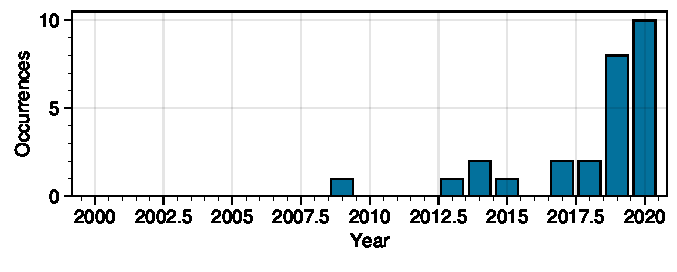
\includegraphics[width=8.3cm]{Figures/methods/Figure_4.pdf}
\caption{French alpine glaciers used for model training and validation and their classification into 3 clusters/regions (Écrins, Vanoise, Mont-Blanc). Coordinates of bottom left map corner: 44º32'N, 5º40'E, coordinates of the top right map corner: 46º08'N, 7º17'E.}
\label{methods:fig4}
\end{wrapfigure}

Glacier ice thickness data come from \citet{farinotti_consensus_2019}, hereafter F19, based on the Randolph Glacier Inventory v6.0 \citep[RGI,][]{consortium_randolph_2017}. The ice thickness values represent the latest consensus estimate, averaging an ensemble of different methods based on the principles of ice flow dynamics to invert the ice thickness from surface characteristics.

We also have ice thickness data acquired by diverse field methods \citep[seismic, ground penetrating radar or hot water drilling,][]{rabatel_estimation_2018} for four glaciers of the GLACIOCLIM observatory. We compared these in situ thickness data, with the simulated ice thicknesses from F19 (refer to Supplements for detailed information). Although differences can be found (locally up to 100\% in the worst cases), no systematic biases were found with respect to glacier local slope nor glacier altitude; therefore, no systematic correction was applied to the dataset. The simulated ice thicknesses for Saint-Sorlin (2 \(km^2\), mean altitude = 2920 m.a.s.l., Écrins cluster) and Mer de Glace (28 \(km^2\), mean altitude = 2890 m.a.s.l., Mont-Blanc cluster) glaciers are  satisfactorily modelled by F19. Mer de Glace's tongue presents local errors of about 50 m, peaking at 100 m (30\% error) around 2000-2100 m.a.s.l, but the overall distribution of the ice is well represented. Saint Sorlin glacier follows a similar pattern, with maximum errors of around 20 m (20\% error) at 2900 m.a.s.l. and a good representation of the ice distribution. The ice thicknesses for Argentière Glacier (12.8 \(km^2\), mean altitude = 2808 m.a.s.l., Mont-Blanc cluster) and Glacier Blanc (4.7 \(km^2\), mean altitude = 3196 m.a.s.l., Écrins cluster) are underestimated by F19 with an almost constant bias with respect to altitude, as seen in \citet{rabatel_estimation_2018}. Therefore, a manual correction was applied to the F19 datasets for these two glaciers based on the field observations from the GLACIOCLIM observatory. A detailed plot (Fig. \ref{methods:figS2}) presenting these results can be found in the supplementary material.

\subsubsection{Climate data}

In our French Alps case study, ALPGM is forced with daily mean near-surface (2 m) temperatures, daily cumulative snowfall and rain. The SAFRAN dataset is used to provide this data close to the glaciers’ centroids. SAFRAN meteorological data \citep{durand_reanalysis_2009} is a reanalysis of weather data including observations from different networks, and specific to the French mountain regions (Alps, Pyrenees and Corsica). Instead of being structured as a grid, data is provided at the scale of massifs, which are in turn divided into altitude bands of 300 meters and into 5 different aspects (north, south, east, west and flat). 

\subsection{Glacier-wide surface mass balance simulations: validation and results} \label{methods:case_study:SMB}

In this section, we go through the selection of SMB predictors, we introduce the procedure for building machine learning SMB models, we assess their performance in space and time and we show some results of simulations using the French alpine glaciers dataset. 

\subsubsection{Selection of predictors}

Statistical relationships between meteorological and topographical variables with respect to glacier-wide SMB are frequent in the literature for the European Alps \citep{hoinkes_glacier_1968}. \citet{martin_correlation_1974} performed a sensitivity study on the SMB of the Saint-Sorlin and Sarennes glaciers (French Alps) with respect to multi-annual meteorological observations for the 1957-1972 period. \citet{martin_correlation_1974} obtained a multiple linear regression function based on annual precipitation and summer temperatures, and he concluded that it could be further improved by differentiating winter and summer precipitations. \citet{six_sensitivity_2014} studied the sensitivity of the SMB to climate change in the French Alps from 1998 until 2014. They found that the variance of summer SMB is responsible for over 90\% of the variance of the annual glacier-wide SMB. \citet{rabatel_changes_2013, rabatel_spatio-temporal_2016} performed an extensive sensitivity analysis of different topographical variables (slope of the lowermost 20\% of the glacier area, mean elevation, surface area, length, minimum elevation, maximum elevation, surface area change and length change) with respect to glacier ELA and annual glacier-wide SMBs of French alpine glaciers. Together with \citet{huss_extrapolating_2012}, who performed a similar study with SMB, the most significant statistical relationships were found for the lowermost 20\% area slope, the mean elevation, glacier surface area, aspect and easting and northing. \citet{rabatel_changes_2013} also determined that the climatic interannual variability is mainly responsible for driving the glacier equilibrium-line altitude temporal variability, whereas the topographical characteristics are responsible for the spatial variations in the mean ELA. 

Summer ablation is often accounted for by means of cumulative positive degree days (CPDD). However, in the vast majority of studies, accumulation and ablation periods are defined between fixed dates (\textit{e.g.}, 1st October - 30th April for the accumulation period in the northern mid-latitudes) based on optimizations. As discussed in \citet{zekollari_statistical_2018}, these fixed periods may not be the best to describe SMB variability through statistical correlation. Moreover, the ablation season will likely evolve in the coming century, due to climate warming. In order to overcome these limitations, we dynamically calculate each year the transition between accumulation and ablation seasons (and vice-versa) based on a chosen quantile in the CPDD. We found higher correlations between annual SMB and ablation-period CPDD calculated using this dynamical ablation season. On the other hand, it was not the case for the separation between summer and winter snowfall. Therefore, we decided to keep constant periods to account for winter (1st October-1st May) and summer (1st May-1st October) snowfalls, and to keep them dynamical for the CPDD calculation.

Following this literature review, vectors $\hat{\Omega}$ and $\hat{C}$ from (Eq. \ref{eq:1}) read as:

\begin{equation} \label{eq:2}
\hat{\Omega}=\left[\begin{array}{lllllll}{\overline{Z}   \quad Z_{\max }   \quad \alpha_{20\%}  \quad \text {Area}  \quad \text{Lat}  \quad \text{Lon }  \quad \Phi }\end{array}\right]
\end{equation}

\begin{equation} \label{eq:3}
\widehat{C}=\left[\begin{array}{lllll}{\Delta C P D D} \quad {\Delta W S} \quad {\Delta S S} \quad {\Delta \overline{T}_{\operatorname{mon}}} \quad {\Delta \overline{S}_{\operatorname{mon}}}\end{array}\right]
\end{equation}
\\ 
Where: \\
$\overline{Z}$: Mean glacier altitude \\
$\quad Z_{\max }$: Maximum glacier altitude \\
$\quad \alpha_{20\%}$: Slope of the lowermost 20\% glacier altitudinal range \\
$Area$: Glacier surface area \\
$Lat$: Glacier latitude \\
$Lon$: Glacier longitude \\
$\Phi$: Cosine of the glacier’s aspect (North = 0º) \\
${\Delta C P D D}$: CPDD (Cumulative Positive Degree Days) anomaly \\
${\Delta W S}$: Winter snow anomaly \\
${\Delta S S}$: Summer snow anomaly \\
${\Delta \overline{T}_{\operatorname{mon}}}$: Average temperature anomaly for each month for the hydrological year \\
${\Delta \overline{S}_{\operatorname{mon}}}$: Average snowfall anomaly for each month for the hydrological year \\

For the linear machine learning models training, we chose a function $f$ that linearly combines $\hat{\Omega}$ and $\hat{C}$, generating new combined predictors (Eq. \ref{eq:4}). In $\hat{C}$, only ${\Delta CPDD}$, ${\Delta WS}$, and ${\Delta SS}$ are combined, to avoid generating an unnecessary amount of predictors with the combination of $\hat{\Omega}$ with ${\Delta \overline{T}_{\operatorname{mon}}}$ and ${\Delta \overline{S}_{\operatorname{mon}}}$.

\begin{equation} \label{eq:4}
\begin{flushleft}
\begin{math}
\begin{aligned}
S M B_{g, y} ={} & ((a_{1} \overline{Z}+a_{2} Z_{\max }+a_{3} \alpha_{20\%}+a_{4} Area+a_{5} Lat+a_{6} L o n+a_{7} \Phi+a_{8}) \Delta CPDD + \\
& (b_{1} \overline{Z}+b_{2} Z_{\max }+b_{3} \alpha_{20\%}+b_{4} Area+b_{5} L a t+b_{6} L o n+b_{7} \Phi+b_{8}) \Delta SS + \\
& (c_{1} \overline{Z}+c_{2} Z_{\max }+c_{3} \alpha_{20\%}+c_{4} Area+c_{5} Lat+c_{6} Lon+c_{7} \Phi+c_{8}) \Delta WS + \\
& d_{1} \overline{Z}+d_{2} Z_{\max }+d_{3} \alpha_{20\%}+d_{4} Area+d_{5} Lat+d_{6} Lon+d_{7} \Phi+d_{8} + d_{n}{\Delta \overline{T}_{\operatorname{mon}}} + d_{m}{\Delta \overline{S}_{\operatorname{mon}}} + \varepsilon )_{\text{g,y}}
\end{aligned}
\end{math}
\end{flushleft}
\end{equation}
\\
32 glaciers over variable periods between 31 and 57 years result in 1048 glacier-wide SMB ground truth values. For each glacier-wide SMB value, 55 predictors were produced following Eq. \ref{eq:4} 33 combined predictors, with ${\Delta \overline{T}_{\operatorname{mon}}}$ and ${\Delta \overline{S}_{\operatorname{mon}}}$ accounting for 12 predictors each, one for each month of the year. All these values combined produce a 1048x55 matrix, given as input data to the OLS and Lasso machine learning libraries. Early Lasso tests (not shown here) using only the predictors from Eq. \ref{eq:2} and \ref{eq:3} demonstrated the benefits of expanding the number of predictors, as it is later shown in Fig. \ref{methods:fig5}. For the training of the ANN, no combination of topo-climatic predictors is done as previously mentioned (Sect. \ref{methods:methods:SMB}), since it is already done internally by the ANN. 

\subsubsection{Causal analysis}

\begin{wrapfigure}{R}{0.55\linewidth}
\centering
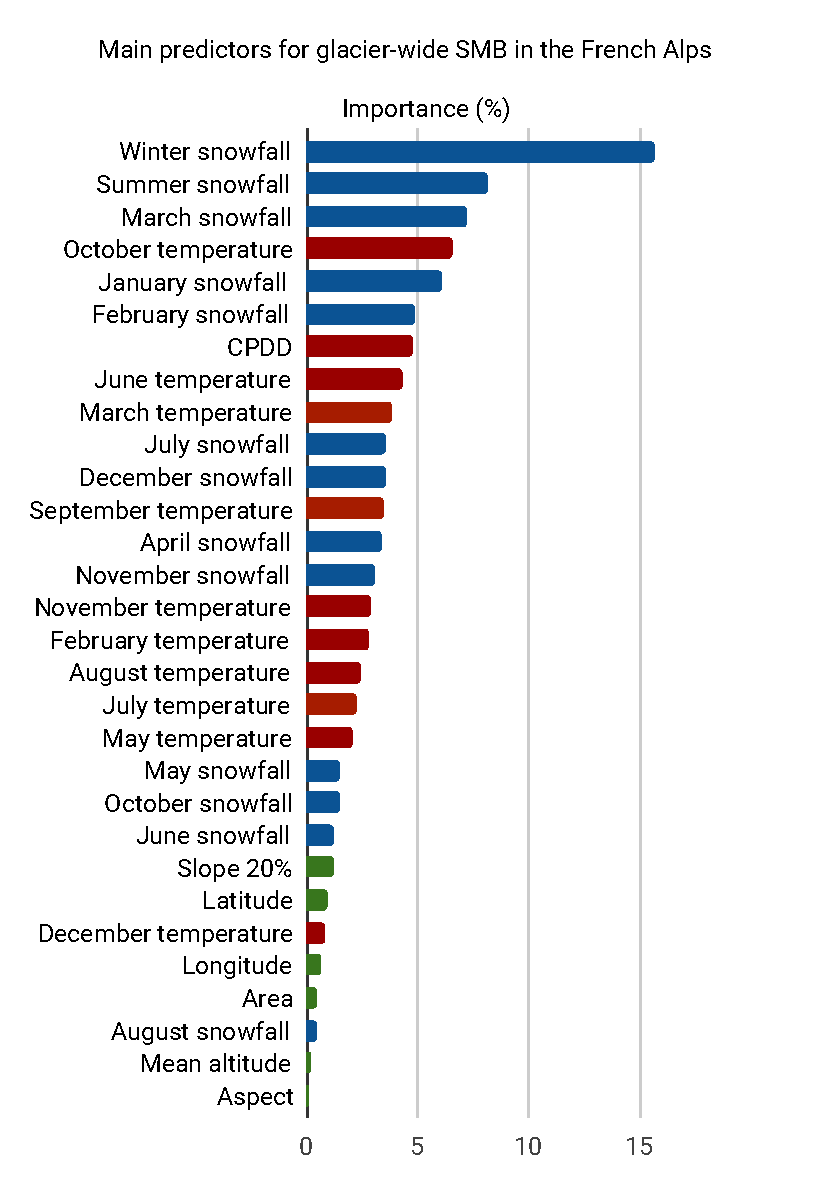
\includegraphics[width=8.3cm]{Figures/methods/Figure_5.pdf}
\caption{Contribution to the total variance of the 30 top topo-climatic predictors out of 55 predictors using Lasso. Green bars indicate predictors including topographical features, blue ones including accumulation-related features, and red ones including ablation-related features}
\label{methods:fig5}
\end{wrapfigure}

By running the Lasso algorithm on the dataset based on Eq. \ref{eq:2} and \ref{eq:3}, we obtain the contribution of each predictor in order to explain the annual glacier-wide SMB variance. Regarding the climatic variables, accumulation-related predictors (winter snowfall, summer snowfall as well as several winter, spring and even summer months), appear as the most important predictors. Ablation-related predictors also seem to be relevant, mainly with CPDD and summer and shoulder season months (Fig. \ref{methods:fig5}). Interestingly, meteorological conditions in the transition months are crucial for the annual glacier-wide SMB in the French Alps: (1) October temperature is determinant for the transition between the ablation and the accumulation season, favouring a lengthening of melting when temperature remains positive, or conversely allowing snowfalls that protect the ice and contribute to the accumulation when temperatures are negative; (2) March snowfall has a similar effect: positive anomalies contribute to the total accumulation at the glacier surface, and a thicker snow pack will delay the snow/ice transition during the ablation season leading to a less negative ablation rate \citep[e.g. Fig. \ref{methods:fig6}b,][]{reveillet_relative_2018}. Therefore, meteorological conditions of these transition months seem to strongly impact the annual glacier-wide SMB variability, since their variability oscillates between positive and negative values, unlike the months in the heart of summer or winter. 

In a second term, topographical predictors do play a role, albeit a secondary one. The slope of the 20\% lowermost altitudinal range, the glacier area, the glacier mean altitude and aspect help to modulate the glacier-wide SMB signal, which unlike point or altitude-dependent SMB, partially depends on glacier topography \citep{huss_conventional_2012}. Moreover, latitude and longitude are among the most relevant topographical predictors, which for this case study are likely to be used as bias correctors of precipitation of the SAFRAN climate reanalysis. SAFRAN is suspected of having a precipitation bias, with higher uncertainties for high altitude precipitations \citep{vionnet_numerical_2016}. Since the French Alps present an altitudinal gradient, with higher altitudes towards the eastern and the northern massifs, we found that the coefficients linked to latitude and longitude enhanced glacier-wide SMBs with a north-east gradient. 

\subsubsection{Spatial predictive analysis}

In order to evaluate the performance of the machine learning SMB models in space, we perform a leave-one-glacier-out (LOGO) cross-validation. For relatively small datasets like the one used in this study, cross-validation ensures that the model is validated on the full dataset. Such validation aims at understanding the model’s performance for predictions on other glaciers for the same time period as during the training. 

An important aspect is the comparison between linear and nonlinear machine learning algorithms used in this study. \citet{steiner_application_2005} already proved that a nonlinear ANN improved the results with respect a classic stepwise multiple linear regression. Here, we draw a similar comparison using more advanced methods for a larger dataset: OLS and Lasso as linear machine learning algorithms and a deep ANN as a nonlinear one. We observed significant differences between OLS, Lasso and deep learning, both in terms of explained variance (\(r^2\)) and accuracy (RMSE) of predicted glacier-wide SMBs. On average, we found improvements between +55\% and +61\% in the explained variance (from 0.49 to 0.76-0.79) using the nonlinear deep ANN compared to Lasso, whereas the accuracy was improved up to 45\% (from 0.74 to 0.51-0.62). This means that 27\% more variance is explained with a nonlinear model in the spatial dimension for glacier-wide SMB in this region (Fig. \ref{methods:fig6}). An interesting consequence of the nonlinearity of the ANN is the fact that it better captures extreme SMB values compared to a linear model. A linear model can correctly approximate the main cluster of values around the median, but the linear approximation performs poorly for extreme annual glacier-wide SMB values. The ANN solves this problem, with an increased explained variance which translates into a better accuracy for extreme SMB values, even without the use of sample weights (Fig. \ref{methods:fig6}). 

\begin{figure*}[t]
\centering
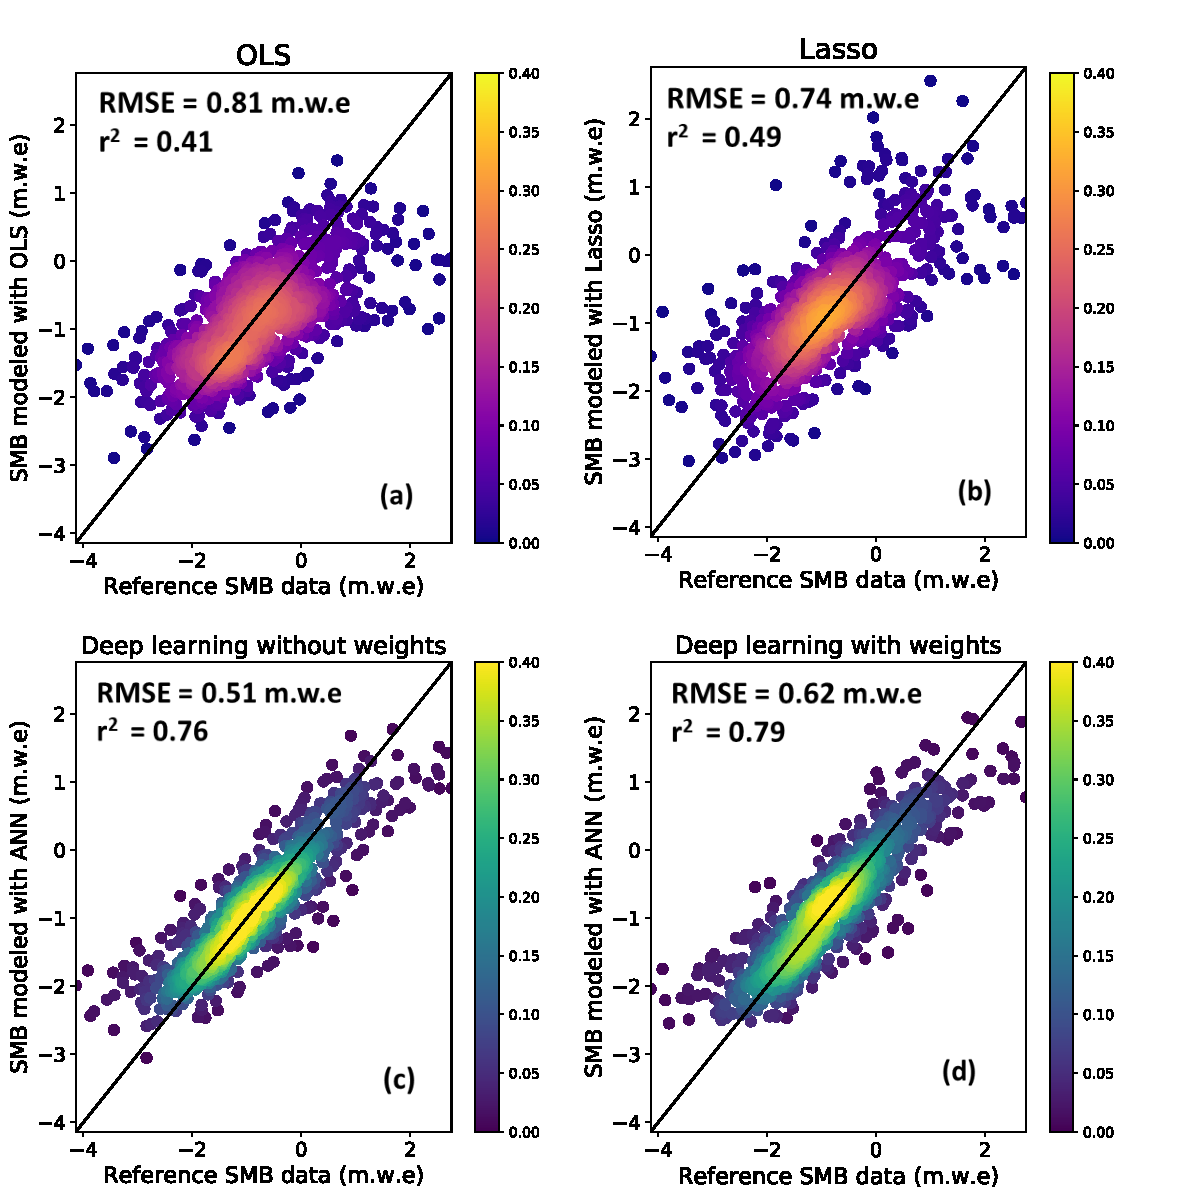
\includegraphics[width=12cm]{Figures/methods/Figure_6.pdf}
\caption{Evaluation of modelled annual glacier-wide SMB against the ground truth SMB data (both in m.w.e. $ a^{-1}$) using Leave-One-Glacier-Out cross-validation. The colour (purple-orange for linear; blue-green for nonlinear) indicates frequency based on the probability density function. The black line indicates the reference one-to-one line. a) Scatter plot of the OLS model results; b) Scatter plot of the Lasso linear model results; Scatter plots of the deep artificial neural network nonlinear models without (c) and with sample weights (d)}
\label{methods:fig6}
\end{figure*}

As a consequence, the added value of deep learning is especially relevant on glaciers with steeper annual changes in glacier-wide SMB (Fig. \ref{methods:fig7}a). The use of sample weights can scale up or down this factor, thus playing with a performance trade-off depending on how much one wants to improve the model’s behaviour for extreme SMB values. 

\begin{figure*}[t]
\centering
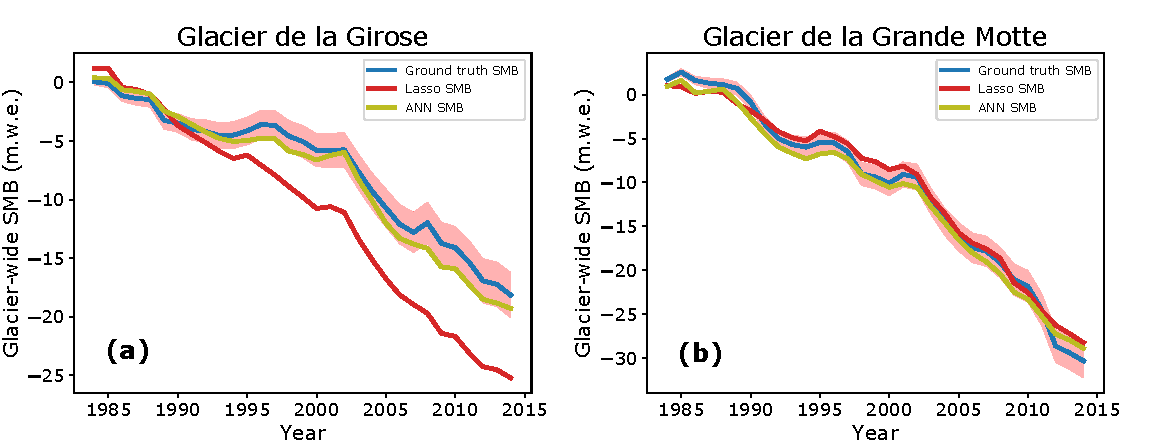
\includegraphics[width=14cm]{Figures/methods/Figure_7.pdf}
\caption{Examples of cumulative glacier-wide SMB (m.w.e.) simulations against the ground truth SMB data. The pink envelope indicates the accumulated uncertainties from the ground truth data. The deep learning SMB model has not been trained with sample weights in these illustrations.}
\label{methods:fig7}
\end{figure*}

Overall, deep learning results in a lower error throughout all the glaciers in the dataset when evaluated using LOGO cross-validation (Fig. \ref{methods:fig8}). Moreover, the bias is also systematically reduced, but it is strongly correlated to the one from Lasso. 

\begin{figure*}[t]
\centering
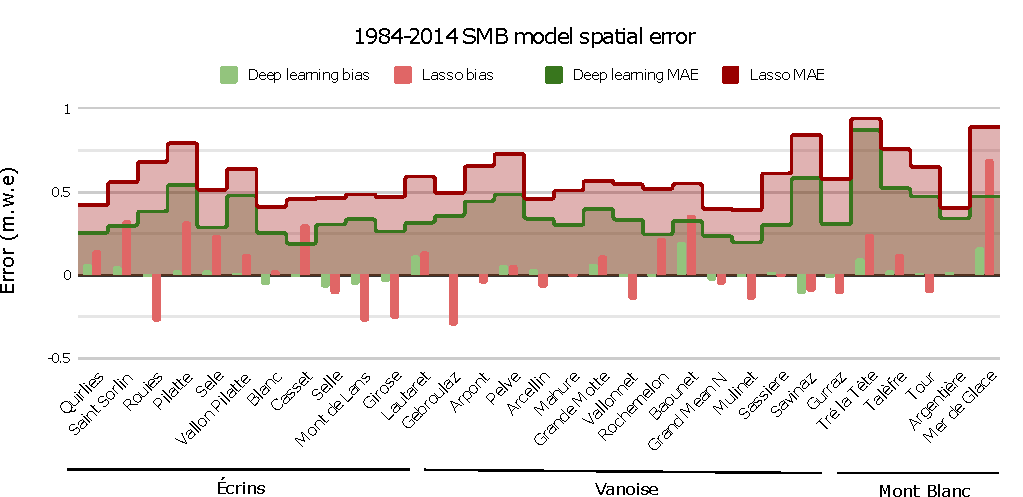
\includegraphics[width=16cm]{Figures/methods/Figure_8.pdf}
\caption{Mean average error (MAE) and bias (vertical bars) for each glacier of the training dataset structured by clusters for the 1984-2014 LOGO glacier-wide SMB simulation. No clear regional error patterns arise}
\label{methods:fig8}
\end{figure*}

\subsubsection{Temporal predictive analysis}

In order to evaluate the performance of the machine learning SMB models in time, we perform a leave-one-year-out (LOYO) cross-validation. This validation serves to understand the model’s performance for past or future periods outside the training time period. The best results achieved for Lasso make no use of any monthly average temperature or snowfall, suggesting that these features are not relevant for temporal predictions unlike the spatial case.

As in Sect. \ref{methods:case_study:SMB}, the results between the linear and nonlinear machine learning algorithms were compared. Interestingly, using LOYO, the differences between the different models were even greater than for spatial validation, revealing the more complex nature of the information in the temporal dimension. As illustrated by Fig. \ref{methods:fig9}, we found remarkable improvements between the linear Lasso and the nonlinear deep learning in both the explained variance (between +94\% and +108\%) and accuracy (between +32\% and +58\%). This implies that 35\% more variance is explained using a nonlinear model in the temporal dimension for glacier-wide SMB balance in this region. Deep learning manages to keep very similar performances between the spatial and temporal dimensions, whereas the linear methods see their performance affected most likely due to the increased nonlinearity of the SMB reaction to meteorological conditions. 

\begin{figure*}[h]
\centering
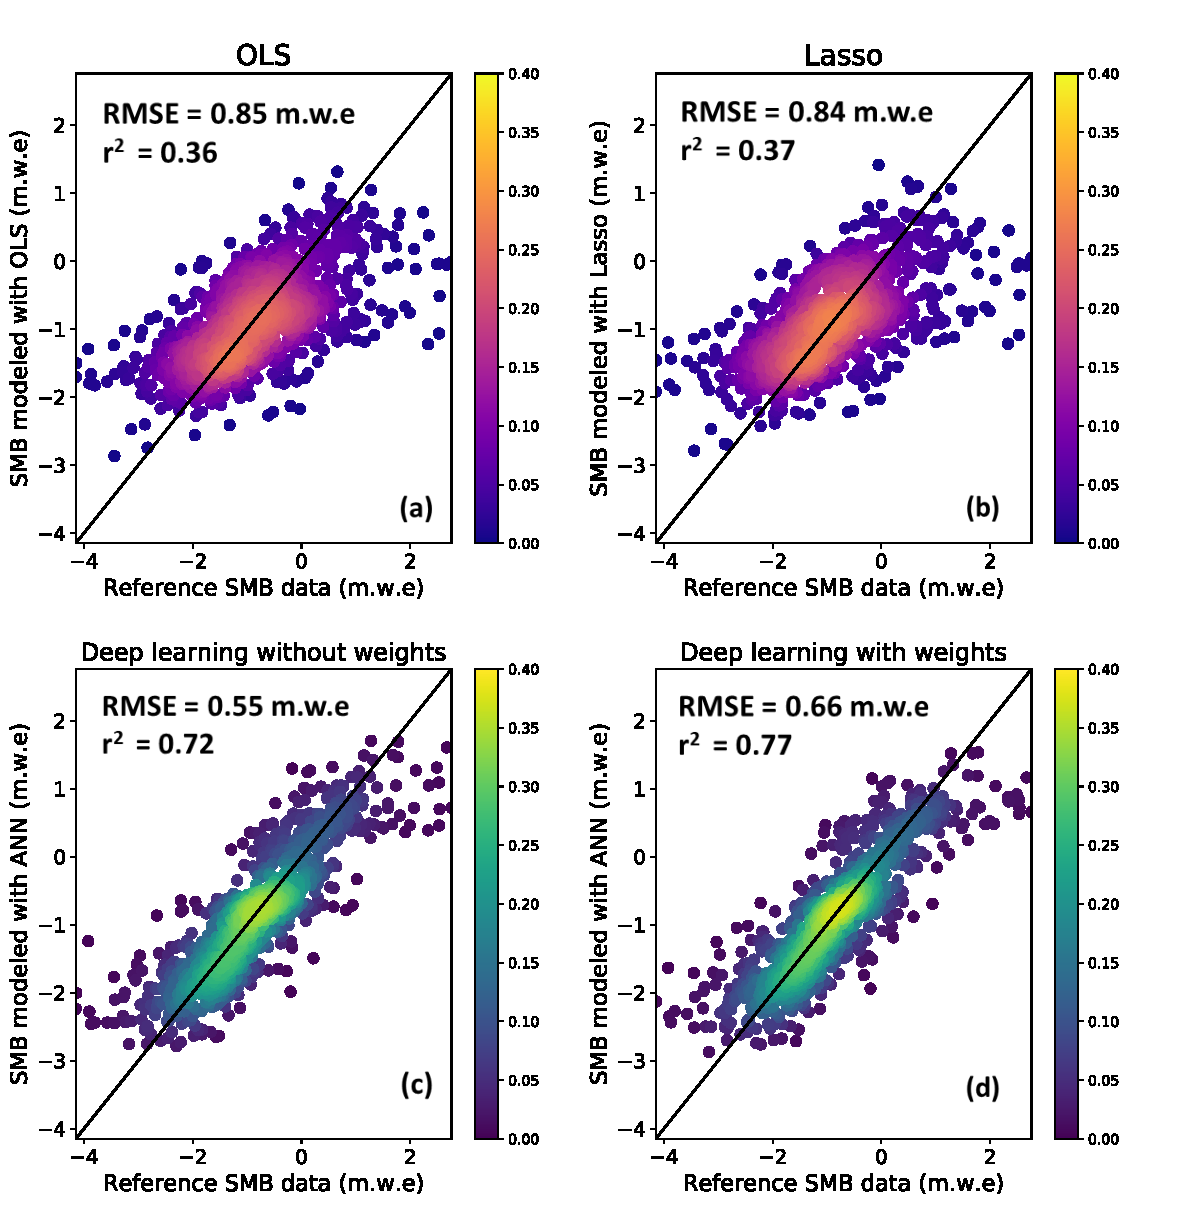
\includegraphics[width=12cm]{Figures/methods/Figure_9.pdf}
\caption{Evaluation of modelled annual glacier-wide SMB against the ground truth SMB data (both in m.w.e. $ a^{-1}$) using Leave-One-Year-Out cross-validation. The colour (purple-orange for linear; blue-green for nonlinear) indicates frequency based on the probability density function. The black line indicates the reference one-to-one line. a) Scatter plot of the OLS model results; b) Scatter plot of the Lasso linear model results; Scatter plots of the deep artificial neural network nonlinear models without (c) and with sample weights (d).}
\label{methods:fig9}
\end{figure*}

A more detailed year by year analysis reveals interesting information about the glacier-wide SMB data structure. As seen in Fig. \ref{methods:fig10}, the years with the worst deep learning precision are 1984, 1985 and 1990. All these three hydrological years present a high spatial variability in observed (or remotely-sensed) SMBs: very positive SMB values in general for 1984 and 1985 with few slightly negative values, and extremely negative SMB values in general for 1990 with few almost neutral values. These complex configurations are clearly outliers within the dataset, which push the limits of the nonlinear patterns found by the ANN. The situation becomes even more evident with Lasso, which struggles to resolve these complex patterns and often performs poorly where the ANN succeeds (\textit{e.g.}, years 1996, 2012 or 2014). The important bias present only with Lasso is representative of its lack of complexity towards nonlinear structures, which results in an underfitting of the data. The average error is not bad, but it shows a high negative bias for the first half of the period, which mostly has slightly negative glacier-wide SMBs, and a high positive bias for the second half of the period, which mostly has very negative glacier-wide SMB values.

\begin{figure*}[t]
\centering
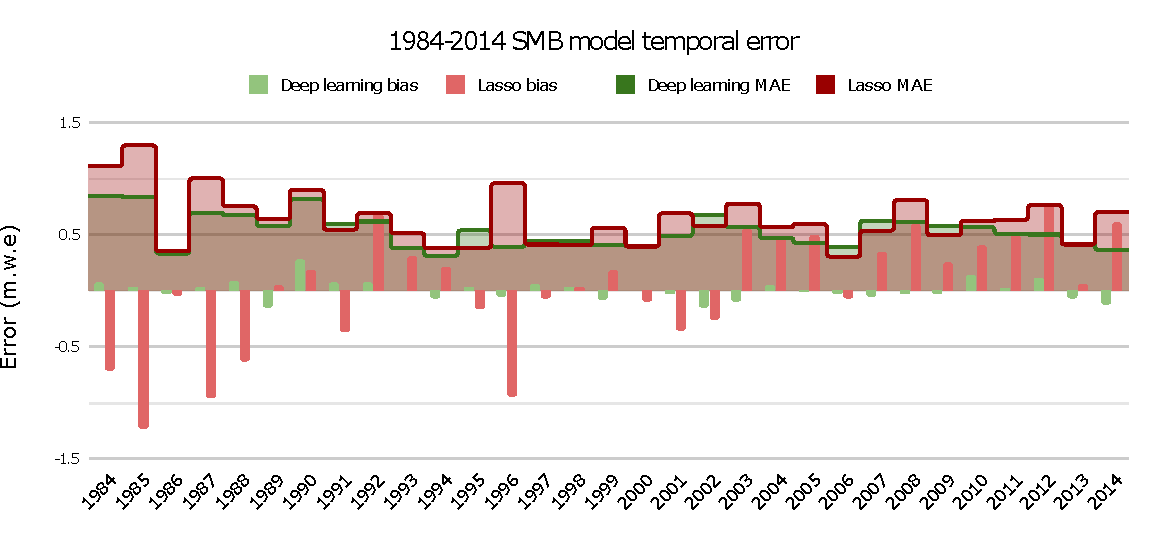
\includegraphics[width=16cm]{Figures/methods/Figure_10.pdf}
\caption{Mean average error (MAE) and bias (vertical bars) for each year of the training dataset for the 1984-2014 LOYO glacier-wide SMB simulation.}
\label{methods:fig10}
\end{figure*}

\subsubsection{Spatiotemporal predictive analysis}

Once the specific performances in the spatial and temporal dimensions have been assessed, the performance in both dimensions at the same time is evaluated using Leave-Some-Years-and-Glaciers-Out (LSYGO) cross-validation. 64 folds were built, with test folds being comprised of data for 2 random glaciers on 2 random years, and train folds of all the data except the 2 years (for all glaciers) and the 2 glaciers (for all years) present in the test fold. These combinations are quite strict, implying that for every 4 tested values we need to drop between 123 and 126 values for training, depending on the glacier and year, to respect the spatiotemporal independence \citep{roberts_cross-validation_2017}. 

The performance of LSYGO is similar to LOYO, with a RMSE of 0.51 m.w.e. and a coefficient of determination of 0.77 (Fig. \ref{methods:figS5}).  This is reflected in the fact that very similar ANN hyperparameters were used for the training. This means that the deep learning SMB model is successful in generalizing and it does not overfit the training data. 

\subsection{Glacier geometry evolution: Validation and results} 
\label{methods:case_study:deltah}

As mentioned in Sect. \ref{methods:methods:deltah}, the Δh parameterization has been widely used in many studies \citep[e.g.,][]{huss_modelling_2008, huss_future_2010, vincent_future_2014, huss_new_2015, huss_global-scale_2018, hanzer_projected_2018, vincent_declin_2019}. It is not in the scope of this study to evaluate the performance of this method, but we present the approach developed in ALPGM to compute the $\Delta$h functions and show some examples for single glaciers to illustrate how these glacier-specific functions perform compared to observations. For the studied French alpine glaciers, the 1979-2011 period is used. This period was proved by \citet{vincent_future_2014} to be representative of Mer de Glace’s secular trend. Other sub-periods could have been used, but it was shown that they did not necessarily improve the performance. In addition, the 1979 and 2011 DEMs are the only ones available that cover all the French alpine glaciers. Within this period, some years with neutral to even positive surface mass balances in the late 1970s and early 1980s can be found, as well as a remarkable change from 2003 onward with strongly negative surface mass balances, following the heatwave that severely affected the western Alps in summer 2003.

The glacier-specific $\Delta$h functions are computed for glaciers $\geq$ 0.5 \(km^2\), which represented about 80\% of the whole glaciarized surface of the French Alps in 2015 (some examples are illustrated in the Supplement Fig. \ref{methods:figS4}). For the rest of very small glaciers (< 0.5 \(km^2\)), a standardized flat function is used in order to make them shrink equally at all altitudes. This is done to simulate the fact that generally, the equilibrium line of very small glaciers has surpassed the glacier’s maximum altitude, thus shrinking from all directions and altitudes in summer. Moreover, due to their reduced size and altitudinal range, the ice flow no longer has the same importance as for larger or medium sized glaciers.

In order to evaluate the performance of the parameterized glacier dynamics of ALPGM, coupled with the glacier-wide SMB component, we compared the simulated glacier area of the 32 studied glaciers with the observed area in 2015 from the most up-to-date glacier inventory in the French Alps. Simulations were started in 2003, for which we used the F19 ice thickness dataset. In order to take into account the ice thickness uncertainties, we ran three simulations with different versions of the initial ice thickness: the original data, -30\% and +30\% of the original ice thickness in agreement with the uncertainty estimated by the authors. Moreover, in order to take into account the uncertainties in the $\Delta$h glacier geometry update function computation, we added a ±10\% variation in the parameterized functions (Fig. \ref{methods:fig11}).

\begin{figure*}[h]
\centering
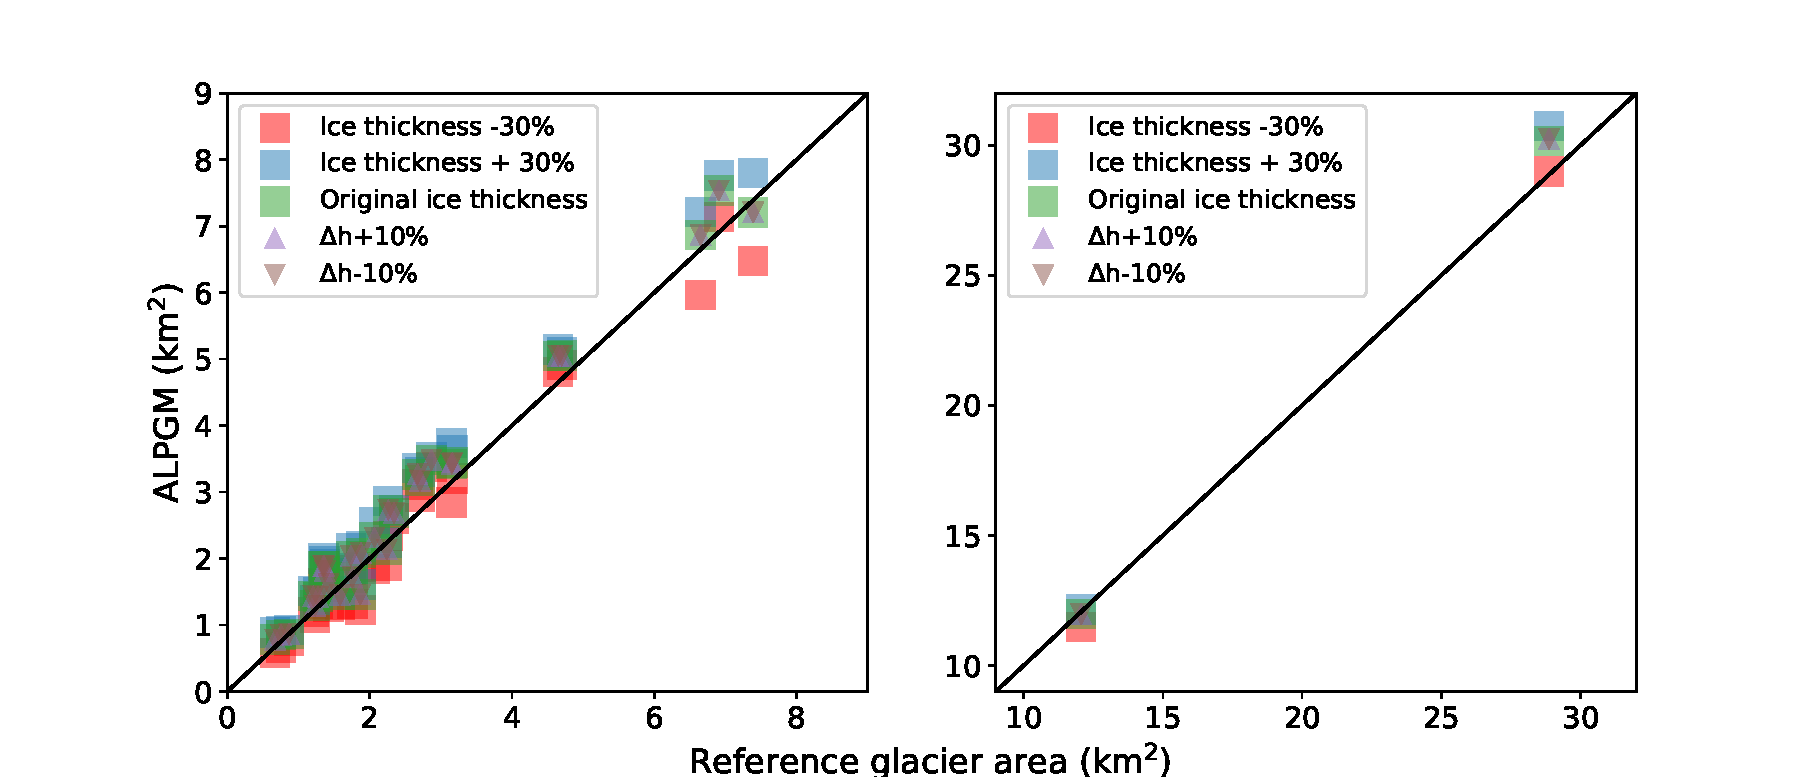
\includegraphics[width=15cm]{Figures/methods/Figure_11.pdf}
\caption{Simulated glacier areas for the 2003-2015 period for the 32 study glaciers using a deep learning SMB model without weights. Squares indicate the different F19 initial ice thicknesses used taking into account their uncertainties and triangles indicate the uncertainties linked to the glacier-specific geometry update functions. For better visualisation, the figure is split in two with the two largest French glaciers on the right.}
\label{methods:fig11}
\end{figure*}

Overall, the results illustrated in Fig. \ref{methods:fig11} show a good agreement with the observations. Even for a 12-year period, the initial ice thickness remains the largest uncertainty, with almost all glaciers falling within the observed area when taking it into account. The mean error in simulated surface area was of 10.7\% with the original F19 ice thickness dataset. Other studies using the $\Delta$h parameterization already proved that the initial ice thickness is the most important uncertainty in glacier evolution simulations, together with the choice of a GCM for future projections \citep{huss_new_2015}. 

\section{Discussion and perspectives} \label{methods:discussion}

\subsection{Linear methods still matter} \label{methods:discussion:linear}

Despite the fact that deep learning often outperforms linear machine learning and statistical methods, there is still a place for such methods in modelling. Indeed, unlike ANNs, simpler regularised linear models such as Lasso allow an easy interpretation of the coefficients associated to each input feature, which helps to understand the contribution of each of the chosen variables to the model. This means that linear machine learning methods can be used for both prediction and causal analysis. Training a linear model in parallel to an ANN has therefore the advantage to provide a simpler linear alternative which can be used to understand the dataset. Moreover, seeing the contribution of each coefficient, one can reduce the complexity of the dataset by keeping only the most significant predictors. Finally, a linear model serves as well as a reference to highlight and quantify the nonlinear gains obtained by deep learning. 

\subsection{Training deep learning models with spatiotemporal data} \label{methods:spatiotemporal}

The creation and training of a deep ANN requires a certain knowledge and strategy with respect to the data and study focus. When working with spatiotemporal data, the separation between training and validation becomes tricky. The spatial and temporal dimensions in the dataset cannot be ignored, and strongly affect the independence between training and validation data \citep{roberts_cross-validation_2017, berlingerio_evaluation_2019}. Depending on how the cross-validation is performed, the obtained performance will be indicative of one of these two dimensions. As it is shown in Sect. \ref{methods:case_study:SMB}, the ANNs and especially the linear modelling approaches had more success in predicting SMB values in space than in time. This is mostly due to the fact that the glacier-wide SMB signal has a greater variability and nonlinearities in time than in space, with climate being the main driver of the annual fluctuations in SMB, whereas geography, and in particular the local topography, modulates the signal between glaciers \citep{huss_extrapolating_2012, rabatel_spatio-temporal_2016, vincent_common_2017}. Consequently, linear models find it easier to make predictions on a given period of time for other glaciers elsewhere in space, than for time periods outside the training. Nonetheless, the deep learning SMB models were capable of equally capturing the complex nonlinear patterns in both the spatial and temporal dimensions. 

In order to cope with the specific challenges related to each type of cross-validation, there are several hyperparameters that can be modified to adapt the ANN’s behaviour. Due to the long list of hyperparameters intervening in an ANN, it is not advisable to select them using brute force with a grid search or cross-validation. Instead, initial tests are performed in a subset of random folds to narrow down the range of best performing values, before moving to the full final cross-validations for the final hyperparameter selection. Moreover, the ANN architecture plays an important role: the number of neurons as well as the number of hidden layers will determine the ANN’s complexity and its capabilities to capture hidden patterns in the data. But the larger the architecture, the higher are the chances to overfit the data. This undesired effect can be counterbalanced using regularization. The amount of regularization (dropout and Gaussian noise in our case, see Sect. \ref{methods:methods:SMB}) used in the training of the ANN necessarily introduces some trade-offs. The greater the dropout, the more we will constrain the learning of the ANN so the higher the generalization will be, until a certain point, where relevant information will start to be lost and performance will drop. On the other hand, the learning rate to compute the stochastic gradient descent, which tries to minimize the loss function, also plays an important role: smaller learning rates generally result in a slower convergence towards the absolute minima, thus producing models with better generalization. By balancing all these different effects, one can achieve the accuracy versus generalization ratio that best suits a certain dataset and model in terms of performance. Nonetheless, one key aspect in machine learning models is data: expanding the training dataset in the future will enable an increase in the complexity of the model and its performance. Consequently, machine learning models see their performance improved as time goes by, with new data becoming available for training. 

Although the features used as input for the model are classical descriptors of the topographical and meteorological conditions of the glaciers, it is worth mentioning that applying the model in different areas or with different data sources would likely require a re-training of the model due to possible biases: different regions on the globe may have other descriptors of importance but also different measuring techniques will likely have different biases. 

\subsection{Perspectives on future applications of deep learning in glaciology} \label{methods:deeplearning}

The currently used meteorological variables in the deep ANN of ALPGM’s SMB component are based on the classic degree-day approach, which relies only on temperature and precipitation. However, the model could be trained with variables involved in more complex models, such as SEB-type models, for which the longwave and shortwave radiation, as well as the turbulent fluxes and albedo intervene. The current model framework allows flexibility in the choice and number of input variables that can reflect different degrees of complexity for the resolved processes. Despite the fact that it has been shown that for glaciers in the European Alps there is almost no added value in transitioning from a simple degree-day to a SEB model for annual glacier-wide SMB simulations \cite[e.g.,][]{reveillet_which_2017}, it could be an interesting way to expand the training dataset for glaciers in tropical and subtropical regions, where shortwave radiation plays a much more important role \citep{benn_glaciers_2014}. \citet{maussion_enso_2015} followed a similar approach with linear machine learning in order to calibrate a regression-based downscaling model that linked local SEB/SMB fluxes to atmospheric reanalysis variables. 

In this work, we also evaluated the resilience of the deep learning approach: since many glacierized regions in the world do not have the same amount of data used in this study, we trained an ANN only with monthly average temperature and snowfall, without any topographical predictors, to see until which point the algorithm is capable of learning from minimal data. The results were quite interesting, with a coefficient of determination of 0.68 (against 0.76 from the full model) and a RMSE of 0.59 m.w.e. $a^-1$ (against 0.51 from the full model). These results indicate that meteorological data is the primary source of information, determining the interannual high frequency variability of the glacier-wide SMB signal. On the other hand, the “bonus” of topographical data helps to  modulate the high frequency climate signal, by adding a low frequency component to better differentiate glaciers and the topographical characteristics included in the glacier-wide SMB data \citep{huss_conventional_2012}. The fact that glacier-wide SMB is influenced by glacier topography poses the question of determining if the simulated glacier geometries can correctly reproduce topographical observations, needed to represent the topographical feedback present in glacier-wide SMB signals. These aspects are analyzed and discussed in Sect. \ref{methods:case_study} of the Supplementary material, showing small differences between the observed and simulated topographical parameters for the 2003-2015 period (Table S1). Additionally, the simulated glacier-wide SMBs using simulated topographical parameters show very small differences (0.069 m.w.e. $a^-1$ on average) compared to simulations using topographical observations (Fig. \ref{methods:figS6}). Since glacier ice thickness estimates date from the year 2003 \citep{farinotti_consensus_2019}, our validation period can only encompass 12 years. According to all the available data for validation, our model seems to be able to correctly reproduce the glacier geometry evolution, but since the 2003-2015 validation period is quite short, the validation performance might not be representative when dealing with future glacier evolution projections of several decades. Consequently, these aspects will have to be taken into account for future studies using this modelling approach for projections. Moreover, the cross-validation results of the SMB model(s) (Fig. \ref{methods:fig6}-\ref{methods:fig10}) are representative of the performance of predictions using topographical observations. Despite the small differences found between simulated and observed topographical parameters, the SMB model's performance might be slightly different than the performance found in the cross-validation analysis. Therefore, it would be interesting for future studies to investigate the use of point SMB data, which could avoid the complexities related to the influence of glacier topography in glacier-wide SMB. 

A nonlinear deep learning SMB component like the one used for ALPGM could provide an interesting alternative to classical SMB models used for regional modelling. The comparison with other SMB models is beyond the scope of this study, but it would be worth investigating to quantify the specific gains that could be achieved by switching to a deep learning modelling approach. Nonetheless, the linear machine learning models trained with the CPDD and cumulative snowfall used in this study behave in a similar way to a calibrated temperature-index model. Even so, we believe that future efforts should be taken towards physics-informed data science glacier SMB and evolution modelling. Adding physical constraints in ANNs, with the use of physics-based loss functions and/or architectures \cite[e.g.,][]{karpatne_physics-guided_2018}, would allow improving our understanding and confidence in predictions, reduce our dependency on big datasets, and to start bridging the gap between data science and physical methods \citep{karpatne_theory-guided_2017, de_bezenac_deep_2018, lguensat_learning_2019, rackauckas_universal_2020}.  Deep learning can be of special interest once applied in the reconstruction of SMB time series. More and more SMB data is becoming available thanks to the advances in remote sensing \citep[e.g.,][]{brun_spatially_2017, zemp_global_2019, dussaillant_two_2019}, but these datasets often cover limited areas and the most recent time period in the studied regions. An interesting way of expanding a dataset would be to use a deep learning approach to fill the data gaps, based on the relationships found in a subset of glaciers as in the case study presented here. Past SMB time series of vast glaciarized regions could thereby be reconstructed, with potential applications in remote glaciarized regions such as the Andes or High Mountain Asia. 

\section{Conclusions} 

We presented a novel approach to simulate and reconstruct glacier-wide SMB series using deep learning for individual glaciers at a regional scale. This method has been included as a SMB component in ALPGM \citep{bolibar_jordibolibar/alpgm:_2019}, a parameterized regional glacier evolution model, following an alternative approach to most physical and process-based glacier models. The data-driven glacier-wide SMB modelling component is coupled with a glacier geometry update component, based on glacier-specific parameterized functions. Deep learning is shown to outperform linear methods for the simulation of glacier-wide SMB with a case study of French alpine glaciers. By means of cross-validation, we demonstrated how important nonlinear structures (up to 35\%) coming from the glacier and climate systems in both the spatial and temporal dimensions are captured by the deep ANN. Taking into account this nonlinearity substantially improved the explained variance and accuracy compared to linear statistical models, especially in the more complex temporal dimension. As we have shown in our case study, deep ANNs are capable of dealing with relatively small datasets, and they present a wide range of configurations to generalize and prevent overfitting. Machine learning models benefit from the increasing number of available data, which makes their performance constantly improve as time goes by. 

Deep learning should be seen as an opportunity by the glaciology community. Its good performance for SMB modelling in both the spatial and temporal dimensions shows how relevant it can be for a broad range of applications. Combined with in situ or remote sensing SMB estimations, it can serve to reconstruct SMB time series for regions or glaciers with already available data for past and future periods, with potential applications in remote regions such as the Andes or the high mountains of Asia. Moreover, deep learning can be used as an alternative to classical SMB models as it is done in ALPGM: important nonlinearities from the glacier and climate systems are potentially ignored by these mostly linear models, which could give an advantage to deep learning models in regional studies. It might still be too early for the development of such models in certain regions which lack consistent datasets with a good spatial and temporal coverage. Nevertheless, upcoming methods adding physical knowledge to constrain neural networks \cite[e.g.,][]{karpatne_physics-guided_2018, rackauckas_universal_2020} could provide interesting solutions to the limitations of our current method. By incorporating prior physical knowledge in neural networks, the dependency on big datasets would be reduced, and it would enable a transition towards more interpretable physics-informed data science models. 

\section{Supplementary material}

\subsection{Filtering of DEM rasters}

Before computing the glacier-specific $\Delta$h parameterized functions, some preprocessing is done to the regional French Alps DEM raster files in order to filter artefacts and noise. The processing chain works as follows:

\begin{enumerate}
 
\item The regional DEM files are cropped using the 2003 glacier inventory shapefile outlines, thus obtaining glacier-specific rasters with the DEMs from 1979 and 2011.
\item The glacier surface altitude difference for this period (so-called dh/dt) which corresponds to the change in ice thickness is computed glacier by glacier by subtracting the two previously mentioned DEM rasters.
\item A first empirical filter is applied to all rasters to filter unrealistic values coming from artefacts (e.g., presence of clouds or saturation on the images used to generate de DEMs).
\item The filtered ice thickness difference (dh/dt) and DEM rasters are paired together as in Figure 12, and a low-order polynomial fit is applied in order to get the main trend of the scatterplot between the ice thickness difference vs. altitude.
\item A dynamic envelope/buffer around the polynomial fit line is computed for each glacier based on a quantile between maximum and minimum values for each altitude. In order to smooth the computed envelope for each altitude, a convolutional filter is applied to these values in order to smooth them and to follow the polynomial fit. A dynamic sliding window size is used to adjust the averaging process to the characteristics of each glacier. 
\item A second filter is then applied using the computed smoothed envelope buffer to remove outliers
\item A final polynomial fit is computed with a variable order depending on the number of remaining data values of each glacier.
\item The percentage of pixels of information available for computing the polynomial fit (the parameterized function) is displayed for each glacier at the end of the processing chain.

\end{enumerate}
 
\subsection{SMB statistical error analysis}

In order to determine the error due to each predictor, a Lasso model was trained with the same training matrix as the ANN, but instead of using SMB as ground truth data the errors generated by the ANN without weights were used. As discussed in section \ref{methods:discussion:linear}, Lasso performs a regularization on the training dataset, thus keeping only certain predictors and removing the rest. By looking at the resulting coefficients of the model, we can estimate the linear contribution of each predictor to the final model error. Latitude and longitude appear as the most important error predictors, but their contribution might in fact indicate the different magnitude of errors between glaciers or regions, since the pair of coordinates specifically identifies each glacier. October, August and March temperature follow behind, indicating that changes in temperature during these months have an influence in the simulation errors. It is not surprising that two of these months appear as top predictors (Fig. \ref{methods:fig5}), as changes in temperature during these months at the transition between the accumulation and ablation season can have a strong importance on the surface mass balance processes. 

\begin{figure*}[h]
\centering
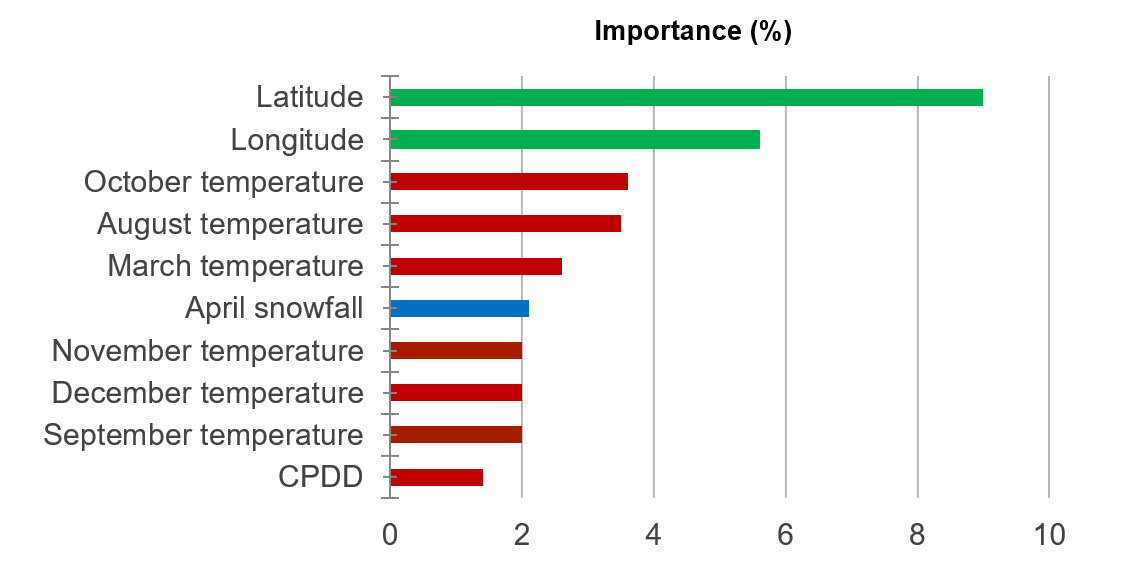
\includegraphics[width=12cm]{Figures/methods/Figure_S1.png}
\caption{Importance (\%) of the first 10 predictors using Lasso to predict residual error from the ANN SMB model. Green bars indicate topographical features, red bars temperature-related features and blue bars precipitation-related features.}
\label{methods:figS1}
\end{figure*}

Such an approach to analyze the influence of the different predictors into the quantification of uncertainties is of course limited, since a linear model is trained with nonlinear results. But these results are useful to determine the main contributors to errors rather than quantifying these errors, which has been done with the LOGO, LOYO and LSYGO cross-validations. 

\subsection{Topographical glacier-wide SMB predictors}

Since topography plays a role in the glacier-wide SMB signal, besides the climate, the representation of the glacier’s topography is important in order to correctly simulate its glacier-wide SMB and its geometrical evolution. As explained in Sect. \ref{methods:methods} “Model overview and workflow” and Sect. \ref{methods:case_study:data} “Topographical glacier data and altimetry”, the source of the topographical predictors used for the simulation of glacier-wide SMB is different at different steps of the glacier evolution simulation chain. Two cases exist:

\begin{enumerate}
 
\item For the machine learning training of the glacier-wide SMB models, which is performed on historical data, all topographical data comes from the multitemporal glacier inventories (Gardent et al., 2014, with 2015 update). In order to have an annual timestep, topographical data from these inventories are linearly interpolated. 
\item For the full glacier evolution simulation, coupling the glacier-wide SMB component with the glacier geometry evolution component, the model must be capable of generating all the input topographical predictors even for non-observed glaciers and future periods. For every glacier and year, all the topographical predictors are computed from the updated glacier-specific ice thickness and DEM raster files from Farinotti et al. (2019), which then are used to simulate a single glacier-wide SMB for that glacier and year. Then, this glacier-wide SMB together with the glacier-specific geometry update function are used to update the glacier’s geometry and their respective ice thickness and DEM rasters. For the next year, all the topographical predictors are recomputed with the updated raster files, and this process is repeated in a loop with an annual timestep. Therefore, the glacier-wide SMB model is called with an annual timestep, simulating only single values in order to take into account the evolution of the glacier’s topography. 

\end{enumerate}

In order to show that the glacier geometry update component, coupled with the glacier-wide SMB simulation component can successfully simulate the evolution of the topographical characteristics of glaciers in the region, a specific test was designed. Using the same validation period as in Sect. \ref{methods:case_study:SMB} (2003-2015), we ran parallel simulations of glacier-wide SMB for all the 32 case study glaciers. The first simulation was done using case (1), with the multitemporal glacier inventories data, and the second one was done following case (2), with the full glacier evolution model and the Farinotti et al. (2019) raster files. The results of both simulations were really similar, revealing only small differences. On average, the simulated glacier-wide SMBs for this period differed on 0.069 m.w.e. a$^{-1}$, due to the differences in the input topographical predictors, which are computed from different datasets (Fig. \ref{methods:figS6}). Moreover, the performances of both simulations for this period are very similar, with a RMSE of 0.49 m.w.e. a$^{-1}$ for case (1) and 0.52 m.w.e. a$^{-1}$ for case (2). The results with all the differences between the simulated glacier-wide SMB values and input topographical values are summarized in Table \ref{methods:tableS1}:

\\

\begin{table}[h!]
\centering
\begin{tabular}{ | m{4cm} | m{2.5cm}| m{1.5cm} | m{4cm} | m{1cm} |} 
 \hline
 Variable (multitemporal inventories vs. full glacier    evolution) & SMB simulated & Slope & Average glacier elevation & Area\\
 \hline MAE or mean difference  & 0.069 m.w.e a$^{-1}$	  & 1.8º	 & 31.3 m & 0.2 km$^{2}$ \\
\hline
\end{tabular}
\caption{Differences on simulated glacier-wide SMB and topographical predictors between a simulation using interpolated topographical predictors from the multitemporal glacier inventories and the full glacier evolution simulations including the coupling of the glacier-wide SMB with the glacier geometry update. }
\label{methods:tableS1}
\end{table}

\\

The only striking difference is perhaps the difference in simulated areas. This is mainly due to the fact that the Farinotti et al. (2019) dataset uses the RGI v6, which for the largest glaciers of Argentière and Mer de Glace, overestimates its surface area (from 32 to 34 km2 for Mer de Glace in 2003). The differences in slope are explained by the fact that this variable is not included in the multitemporal glacier inventories (Gardent et al., 2014), therefore it has been computed once with a global DEM and kept constant for each glacier throughout the years for the training of the SMB model. On the other hand, in order to include the long term effects of glacier morphology changes in the glacier evolution simulations (glacier-wide SMB simulation + glacier geometry update), the glacier slope is re-computed with an annual timestep and it evolves through time. Therefore, there are small differences for certain glaciers whose slope has evolved during this period, thus accounting for the differences with the fixed value used for the training of the SMB model.
 
This test serves to prove that the full glacier evolution simulations in ALPGM are capable of reproducing the topographical predictors used for the training of the glacier-wide SMB machine learning models. Moreover, this test also helps to prove that ALPGM can correctly simulate the topographical evolution of glaciers, which allows to capture the topography induced feedback, which plays a role in the simulation of glacier-wide SMBs. 

\subsection{Supplementary figures}

\begin{figure*}[h]
\centering
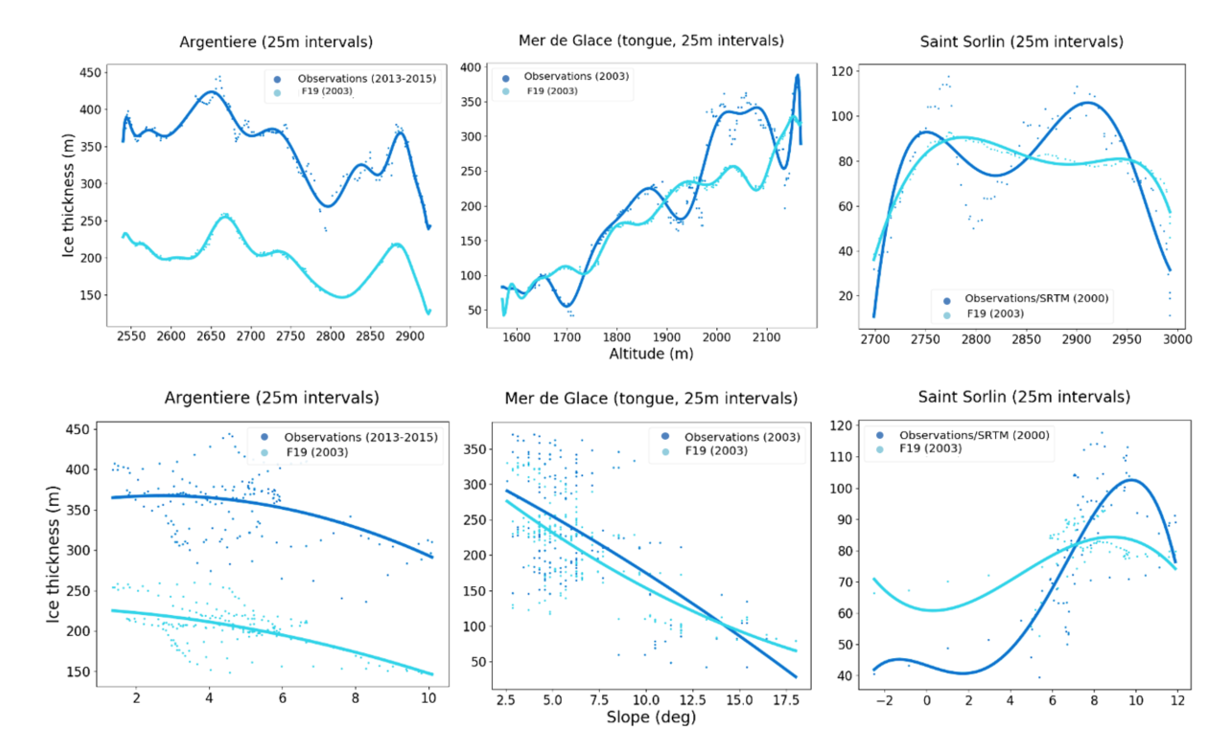
\includegraphics[width=15cm]{Figures/methods/Figure_S2.png}
\caption{Comparison of simulated glacier ice thicknesses from F19 with observations from the GLACIOCLIM observatory. Points are compared at 25 m intervals on the glacier flowline. The polynomial fits have less degrees of freedom for the slope plots. Note that for some glaciers the dates are not the same}
\label{methods:figS2}
\end{figure*}

\begin{figure*}[h]
\centering
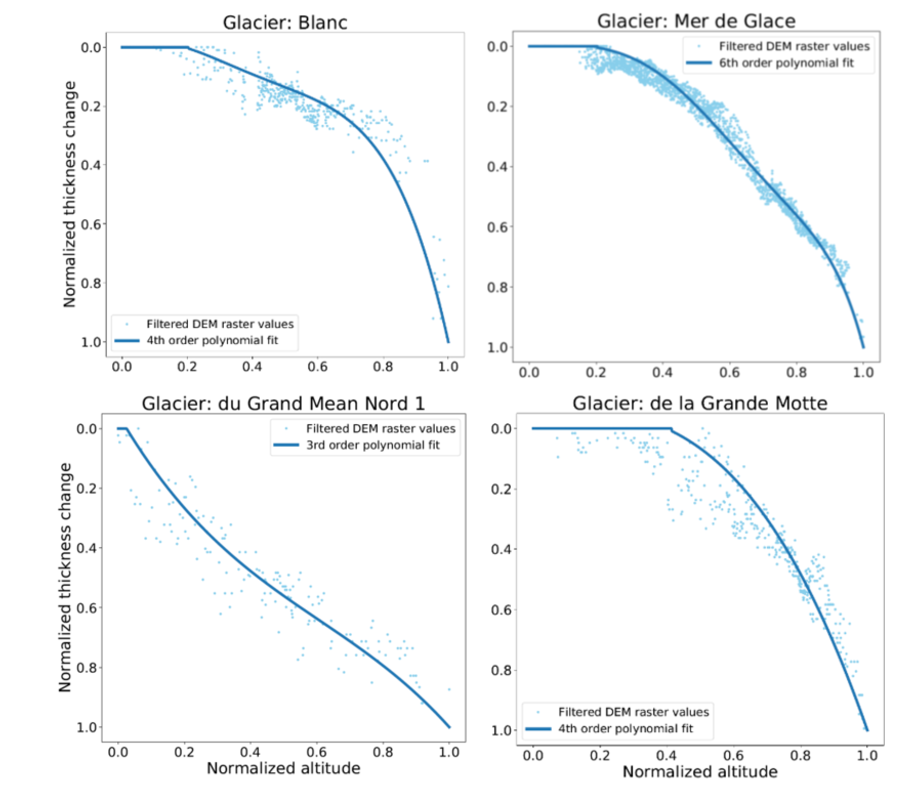
\includegraphics[width=14cm]{Figures/methods/Figure_S3.png}
\caption{Examples of glacier specific $\Delta$h parameterized functions generated by ALPGM. The order of the polynomial fit depends on the number of available pixels.}
\end{figure*}

\begin{figure*}[h]
\centering
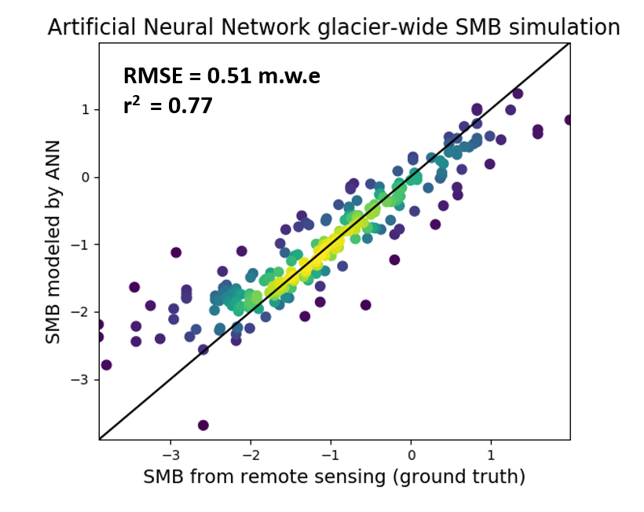
\includegraphics[width=9cm]{Figures/methods/Figure_S4.png}
\caption{Results for the spatiotemporal cross-validation using Leave-Some-Glaciers-and-Years-Out (LSYGO). SMB values are in m.w.e. Compared to the other scatter plots from 3.2, there are less values available for test due to the severity of the spatiotemporal independence.}
\label{methods:figS4}
\end{figure*}

\begin{figure*}[h]
\centering
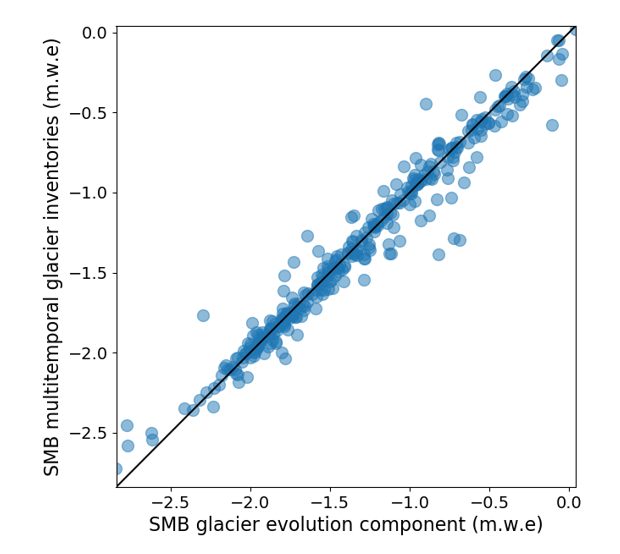
\includegraphics[width=9cm]{Figures/methods/Figure_S5.png}
\caption{Comparison of glacier-wide SMB simulations (2003-2015, 32 case study glaciers) using topographical predictors from the multitemporal glacier inventories (Y axis) vs. using the full glacier evolution simulations in ALPGM with the Farinotti et al. (2019) ice thickness and DEM rasters (X axis). Average difference = 0.069 m.w.e.  a$^{-1}$}
\label{methods:figS5}
\end{figure*}

\begin{figure*}[h]
\centering
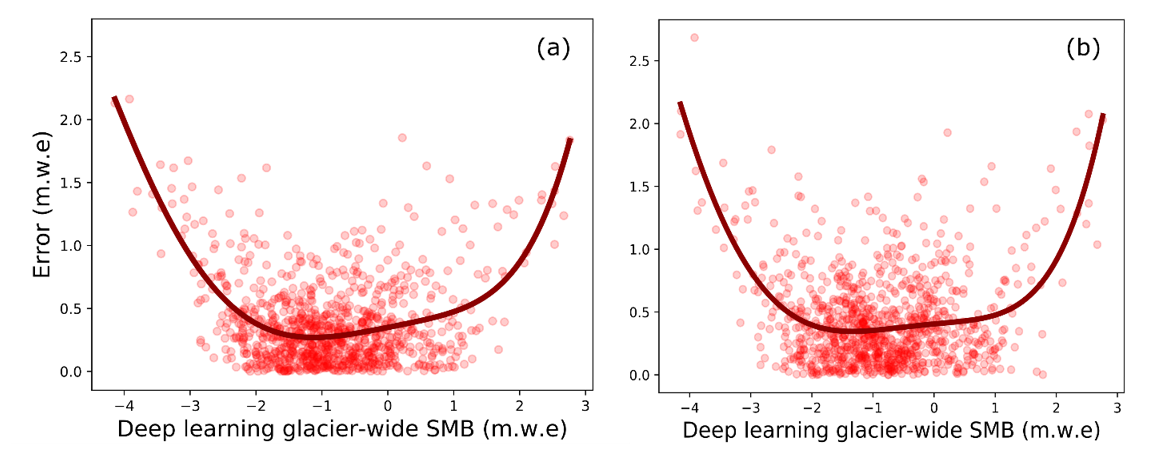
\includegraphics[width=15cm]{Figures/methods/Figure_S6.png}
\caption{Error distribution of deep learning (without weights) glacier-wide SMB simulations for the 1984-2015 period for the 32 case study glaciers. (a) Performance in the spatial dimension using LOGO cross-validation; (b) performance in the temporal dimension using LOYO cross-validation. The red line corresponds to a 5th order polynomial fit.}
\label{methods:figS6}
\end{figure*}
 

